% PVLDB Vol. 20 (VLDB 2027) submission. Official template:
% https://github.com/vldbproceedings/VLDB-Template (acmart.cls v2.19, pvldb.sty v1.0)
\documentclass[sigconf, nonacm]{acmart}

%%% do not modify the following VLDB block %%
%%% VLDB block start %%%
\usepackage{pvldb}% VLDB/PVLDB formatting overrides, see pvldb.sty for details.
%%% VLDB block end %%%

%%%PACKAGES
\usepackage{listings}
\usepackage{xcolor} % Optional: for colors
\usepackage{fancybox} % for \shadowbox used by review comment macros
\usepackage{soul}   % For multi-line highlighting
\let\Bbbk\relax  % Fix for \Bbbk already defined
\usepackage{amssymb, amsmath}
\usepackage{enumitem}
\usepackage{multirow}
\usepackage{tabularx}
\usepackage{booktabs}
% In your preamble:
\usepackage{threeparttable}
\usepackage{algorithm}
\usepackage{algpseudocode} % defines \Require, \Ensure, \State, etc.
\usepackage{makecell} 

\algnewcommand\Input{\item[\textbf{Input:}]}
\algnewcommand\Output{\item[\textbf{Output:}]}

\newcommand{\todo}[1]{\textcolor{red}{[TODO: #1]}}

\newcommand{\hlc}[2][yellow]{{%
    \colorlet{foo}{#1}%
    \sethlcolor{foo}\hl{#2}}%
}


% Define colors
\definecolor{keywordcolor}{rgb}{0,0,0.6}
\definecolor{stringcolor}{rgb}{0.58,0,0.82}
\definecolor{commentcolor}{rgb}{0.4,0.4,0.4}

%colors comentarios
\definecolor{almeidacolor}{rgb}{1,1,0.7}      % Light yellow
\definecolor{altcolor}{rgb}{0.9,1,0.9}   % Light green
\definecolor{penacolor}{rgb}{1,0.9,0.9}    % Light red

\definecolor{maroon(x11)}{rgb}{0.69, 0.19, 0.38}
\definecolor{mangotango}{rgb}{1.0, 0.51, 0.26}

\definecolor{yesbg}{RGB}{198,219,239}      % light desaturated blue
\definecolor{nobg}{RGB}{252,187,161}       % light salmon red
\definecolor{contextbg}{RGB}{254,217,142}  % pale orange
\definecolor{neutralbg}{gray}{0.9}

\definecolor{accent1}{RGB}{198,219,239}   % light blue
\definecolor{accent2}{RGB}{158,202,225}   % medium blue

\newcommand{\csquare}[1]{\colorbox{#1}{\rule{0.8ex}{0.8ex}}}


% requires: \usepackage{tikz}


\newcommand{\na}{n/a}

% SQL style
\lstdefinelanguage{SQL}{
  morekeywords={
    SELECT, FROM, WHERE, AND, OR, NOT, NULL, AS, ON, IN, EXISTS,
    INNER, LEFT, RIGHT, FULL, OUTER, JOIN, GROUP, BY, ORDER, HAVING,
    DISTINCT, UNION, ALL, INSERT, INTO, VALUES, UPDATE, SET, DELETE,
    CREATE, TABLE, PRIMARY, KEY, FOREIGN, REFERENCES, DROP, ALTER, ADD
  },
  sensitive=true,
  morecomment=[l]--,
  morestring=[b]',
}

\lstset{
  language=SQL,
  basicstyle=\small\ttfamily,
  keywordstyle=\color{keywordcolor}\bfseries,
  commentstyle=\color{commentcolor}\itshape,
  stringstyle=\color{stringcolor},
  showstringspaces=false,
  breaklines=true,
  frame=single,
  tabsize=2,
  captionpos=b
}

%% definitions
\newtheorem{problem}{Problem}
\newtheorem{example}{Example}
\newcommand{\D}{\mathcal{D}}       % Dataset
\newcommand{\T}{\mathcal{T}}       % Text corpus
\newcommand{\R}{\mathcal{R}}       % Rules
\newcommand{\Schem}{\mathcal{S}}   % Schema
\newcommand{\FD}{\mathsf{FD}}      % Functional dependency
\newcommand{\IND}{\mathsf{IND}}    % Inclusion dependency
\newcommand{\DC}{\mathsf{DC}}      % Denial constraint
\newcommand{\CK}{\mathsf{CK}}      % Check constraint
\newcommand{\system}{\texttt{Norma}}  
\newcommand{\m}[1]{\mathtt{#1}} % to change a bit






\newif\ifshowcomments
\showcommentstrue  % Change to \showcommentsfalse to disable all
%\showcommentsfalse
% Enable/disable commands
\newcommand{\commenton}{\showcommentstrue}
\newcommand{\commentoff}{\showcommentsfalse}
% Peer commands - now with names, multi-line support, complete disappearing, and different font
\newcommand{\pena}[1]{\ifshowcomments\sethlcolor{penacolor}\hl{\textit{\textbf{Pena: #1}}}\fi}
\newcommand{\alt}[1]{\ifshowcomments\sethlcolor{altcolor}\hl{\textit{\textbf{Alt: #1}}}\fi}
\newcommand{\almeida}[1]{\ifshowcomments\sethlcolor{almeidacolor}\hl{\textit{\textbf{Almeida: #1}}}\fi}

% Review comment macros (same family used in our other papers).
% \altic{...} renders a blue shadowbox note labeled ALTI. To disable all
% comments, redefine \mycomment to {} (see the toggle line below).
\newcommand{\blue}[1]{\textcolor{blue}{#1}}
\newcommand{\mycomment}[2]{\newline\noindent\shadowbox{\begin{minipage}{\dimexpr0.98\columnwidth-\shadowsize-2\fboxrule-2\fboxsep}\textbf{#1: #2}\end{minipage}}}
% \renewcommand{\mycomment}[2]{} % uncomment to hide all comments
\newcommand{\altic}[1]{\blue{\mycomment{ALTI}{#1}}}

% ---------------------------------------------------------------------
% Diff/revision macros, ported from the DesJoin paper preamble.
% Included by Altigran S. da Silva on 2026-08-26.
%
% Usage:  \add{new text}      -> new text, in blue
%         \subs{old}{new}     -> old struck out in red, arrow, new in blue
%         \rem{old text}      -> struck out in red
%         \comm{side remark}  -> prominent review comment
%
% Switch \Reviewtrue to \Reviewfalse below to collapse everything to the
% clean text: \add prints normally, \subs prints only the new text, and
% \rem and \comm vanish. The \altic/\mycomment boxes are NOT governed by
% this switch; they keep their own toggle further up in this file.
% ---------------------------------------------------------------------
\newif\ifReview
\Reviewfalse % change to \Reviewfalse for clean text
\usepackage[normalem]{ulem} % normalem: keep \emph as italics, not underline
\definecolor{commgreen}{rgb}{0.0,0.5,0.0}
\providecommand{\red}[1]{\textcolor{red}{#1}}
\providecommand{\green}[1]{\textcolor{commgreen}{#1}}
\ifReview
    \newcommand{\add}[1]{\textcolor{blue}{#1}}
    \newcommand{\subs}[2]{\red{\sout{#1}}$\rightarrow$\blue{#2}}
    % Updated by Altigran S. da Silva on 2026-08-26: make comments prominent
    % and keep them separate from the surrounding paragraph.
    \newcommand{\comm}[1]{%
      \par\smallskip\noindent
      \fcolorbox{red}{yellow}{%
        \parbox{\dimexpr\columnwidth-2\fboxsep-2\fboxrule}{%
          \textcolor{red}{\textbf{[COMMENT: #1]}}%
        }%
      }%
      \par\smallskip
    }
    \newcommand{\rem}[1]{\red{\sout{#1}}}
\else
    \newcommand{\add}[1]{{#1}}
    \newcommand{\subs}[2]{{#2}}
    \newcommand{\comm}[1]{}
    \newcommand{\rem}[1]{}
\fi


\renewcommand\vldbdoi{XX.XX/XXX.XX}
\renewcommand\vldbpages{XXX-XXX}
% leave empty if no availability url should be set
\renewcommand\vldbavailabilityurl{https://github.com/EduardoPena/norma-text-to-constraints}

\begin{document}

\title{Text-to-Constraints: Mapping Regulatory Requirements to Executable Data Quality Constraints (Extended Version)}

\author{Eduardo H. M. Pena}
\affiliation{%
  \institution{Federal University of Technology-Paraná}
  \country{Brazil}
  \city{Campo Mourão}}
  
\email{eduardo@utfpr.br}

\author{Junio de Freitas}
\affiliation{%
  \institution{Federal University of Amazonas}
  \country{Brazil}
  \city{Manaus}}
\email{junio.freitas@icomp.ufam.edu.br}

\author{Eduardo Cunha de Almeida}
\affiliation{%
  \institution{Federal University of Paran\'{a}}
  \country{Brazil}
  \city{Curitiba}}
\email{eduardo@ufpr.br}

\author{Altigran da Silva}
\affiliation{%
  \institution{Federal University of Amazonas}
  \country{Brazil}
  \city{Manaus}}
\email{alti@icomp.ufam.edu.br}



\begin{abstract}
Many regulatory documents specify requirements that valid data must satisfy, but those specifications are rarely available as data quality constraints. 
%%% texto 'antigo'
%When constraints are missing, the standard solution is constraint discovery, which discovers patterns in the data but cannot recover requirements derived from governing text. 
%When constraints are undefined, a well-studied solution is constraint discovery, but discovery finds patterns the data happens to satisfy, not the requirements it is supposed to satisfy. 
Data profiling, particularly constraint discovery, is a well-studied alternative when constraints are unavailable, but discovered constraints reflect what the data \add{(approximately) }satisfies rather than what it is \subs{supposed}{required} to satisfy.
We introduce the \emph{Text-to-Constraints} problem: given a dataset and related regulatory text, \subs{extract executable data quality constraints grounded in that text}{map the requirements stated in that text to executable data quality constraints over the dataset schema}. 
Then, we present the first framework to address this problem, \system, which identifies verifiable requirements in regulatory documents and maps them to denial constraints using a rich schema-grounded predicate vocabulary. 
We evaluate \system\ on \subs{real-world datasets}{six datasets} with diverse textual and data characteristics, covering constraints ranging from simple checks to complex cross-record rules. \subs{Across constraint classification, extraction, and violation detection, \system\ outperforms baselines from data profiling and Text-to-SQL,}{\system\ outperforms baselines from data profiling and Text-to-SQL in constraint extraction on every dataset on which they were evaluated, and in classification and violation detection on most of them,} recovering constraints they miss and identifying real regulatory violations \rem{with high precision }in publicly released data\add{, including two large mortgage datasets with up to one million records}.







%Data quality constraints (aka data rules) are critical for high-quality, consistent data, yet datasets from data lakes, open data portals, and heterogeneous systems often lack them. Data profiling discovers constraints directly from data but cannot distinguish coincidental patterns from semantically meaningful rules. We pursue a different approach: extracting constraints for a dataset from the regulatory documents relevant to it. However, automated extraction is challenging because constraint sentences are mixed among definitions, procedures, and context, and regulatory text expresses data quality constraints with varied phrasing, implicit scope qualifiers, and conditional logic that must be correctly interpreted to produce executable constraints.
%
%
%
%We introduce the \emph{Text-to-Constraints} problem and present \system\ (\emph{\underline{Norma}tive Constraint Mapper}), a framework for extracting data quality constraints from regulatory text to validate datasets against their regulations. 
%To achieve high accuracy while scaling to large documents, \system\ decomposes the problem into constraint classification and constraint mapping, enabling implementations with different cost-accuracy trade-offs at each stage.
%The most effective configurations combine language models with novel techniques that link passages to schema-grounded constraints.
%We release annotated benchmarks that range from simple checks to complex business rules with conditionals and cross-record dependencies, along with metrics for extraction correctness and violation detection. Experiments show that \system\ outperforms baselines from data profiling, text-to-SQL, and data cleaning, extracting more accurate constraints and identifying more inconsistencies while scaling to large documents at low cost.



%Data quality constraints (or data rules) are key for reliable data, yet datasets from data lakes, open data sources, and heterogeneous systems often lack them.
%%Since manual definition is time-consuming and error-prone, 
%Data profiling aims to discover data rules directly from data; however, current solutions cannot distinguish coincidental patterns from meaningful data rules. We explore a different direction: many datasets have accompanying textual content, for instance, regulatory documents, policy manuals, and legal texts, which implicitly encode data rules. The challenge is that this kind of text does not explicitly state these rules and often mixes them with other content, making them easy to overlook.

%Data quality constraints (or rules) are essential for reliable data, yet datasets from data lakes, open data portals, and heterogeneous systems often lack them. Data profiling discovers constraints directly from data, but cannot distinguish coincidental patterns from semantically meaningful rules. We pursue a different direction: extracting constraints from text. Regulatory documents, policy manuals, and legal texts often define critical data quality rules but the challenge is how to extract,these they rarely explicitly state constraints, mixing them with other content and making extraction difficult.






%In this paper, we introduce the \emph{Text-to-Constraints} problem and present \system\ (\emph{\underline{Norma}tive Constraint Mapper}), a framework that, given a regulatory document and a related dataset, extracts data quality constraints that validate the data. We release annotated datasets targeting expressive constraints, ranging from simple checks to complex business rules with conditionals and multi-record dependencies. We also propose evaluation metrics for the correctness of constraint extraction and the effectiveness of constraint violation detection.
%To handle large documents and datasets, \system\ decomposes the problem into constraint classification and constraint mapping, and supports implementations with different cost-effectiveness trade-offs at each stage. 
%The most effective implementations leverage language models combined with constraint patterns grounded in the schema and data for better constraint extraction. \system\ outperforms diverse baselines in data profiling, text-to-SQL, and data cleaning, consistently extracting more accurate constraints and identifying more data inconsistencies, while scaling to larger documents and datasets at low cost.









\end{abstract}



\maketitle

%%% do not modify the following VLDB block %%
%%% VLDB block start %%%
\vldbtopmatter
%%% VLDB block end %%%

\section{Introduction}
\label{sec:intro}

Many data management tasks rely on \emph{data quality constraints}, which define what constitutes valid data.
However, such constraints are often missing, incomplete, or outdated in real-world datasets. This gap has motivated a large body of work on \emph{data profiling}, where data constraints are automatically discovered from the data itself~\cite{profSurveyFelix2015}. 
Profiling algorithms extract constraints, such as functional dependencies (FDs) and denial constraints (DCs), by identifying patterns that hold over a given data instance, and have been widely used to support data cleaning and error detection~\cite{dependencyTree2020}.

\subs{However, a fundamental assumption underlying this line of work is that constraints must be inferred from data, and thus, they are limited to discovering constraints that reflect what the data \emph{happens to satisfy}, not what it is \emph{required to satisfy}, given some policy, regulation, or legislation. No profiling algorithm can make that distinction, nor can it surface constraints that must hold by design but are violated in the data.}{However, this line of work derives constraints only from the data. Exact discovery returns rules that the instance satisfies, approximate discovery tolerates a fraction of violations~\cite{Pena2019DiscoveryDC,martin2026lima}, and rule-discovery systems help experts rank and refine the candidates~\cite{fan2023topk}. In all cases, the candidates are patterns that hold, exactly or approximately, in the data, rather than rules that the data is \emph{required to satisfy} by some policy, regulation, or legislation. A required rule that is widely violated in the released data is therefore hard to recover from the data alone.}


Many datasets are governed by rules specified in regulatory documents, policy manuals, and operational specifications, which define requirements such as mandatory fields, valid values, eligibility criteria, uniqueness conditions, quotas, and ordering rules~\cite{batini2009methodologies,serra2024IQcontextDtaQuality,CABALLERO2022102058}. Formalizing these rules as constraints is difficult because they depend on combinations of attributes, relationships across tuples, comparison operators, thresholds, and context-dependent conditions, requiring expressive \emph{data quality constraints}. However, since such rules are typically expressed only in natural language, they are rarely translated into executable constraints and used with the data they govern. Consequently, datasets are frequently released without an explicit representation of their own correctness requirements, so violations remain undetected and subsequent analyses may be based on data that does not satisfy their intended specification.

\rem{This problem is common in modern data settings, where open-data portals publish standalone files with limited metadata, data lakes aggregate heterogeneous sources, and data pipelines connect systems whose semantics are only partially documented~\mbox{\cite{datasetSearch2020,Governor2023}}.}


\begin{example}[Brazilian public university admission]
\label{ex:intro}
Brazil's ``Sistema de Sele\c{c}\~{a}o Unificada'' (SISU) manages the public university placements for millions of students annually. The application data is publicly available,\footnote{\url{https://dadosabertos.mec.gov.br/sisu}} with sensitive fields anonymized. The dataset schema includes attributes such as \emph{student\_id}, \emph{course\_code}, \emph{shift}, \emph{institution\_id}, \emph{year}, and \emph{edition}. The rules that define correct enrollment outcomes, however, are described in separate documents that do not accompany the dataset. For instance, Normative Ruling No.\ 21/2012\footnote{\url{https://sisugestao.mec.gov.br/docs/portaria-2012-21.pdf}} is a PDF file found on the Brazilian government website that states (Article 19):\footnote{Schema elements and quoted statements translated from Portuguese for readability.}

\begin{quote}
\textit{``$\ldots$ the student will be ranked in descending order of scores for the seat option they applied to, respecting the available seats at the institution, by campus location, course, and shift, as well as the student's admission category\subs{..}{.}''}
\end{quote}

This passage defines an \emph{ordering constraint}: within each context defined by institution, campus, course, shift, and admission category (and per year/edition), a higher score should not result in a worse rank. The following SQL query checks for violations of this requirement in SISU's application data:

\begin{lstlisting}[language=SQL, frame=none, basicstyle=\footnotesize\ttfamily, mathescape]
SELECT t.student_id, t$^\prime$.student_id
  FROM applications t, applications t$^\prime$
 WHERE t.student_id <> t$^\prime$.student_id
   -- same context
   AND t.year = t$^\prime$.year
   AND t.edition = t$^\prime$.edition
   AND t.institution_id = t$^\prime$.institution_id
   AND t.campus_id = t$^\prime$.campus_id
   AND t.course_code = t$^\prime$.course_code
   AND t.shift = t$^\prime$.shift
   AND t.application_mode = t$^\prime$.application_mode
   -- violation: higher score but worse ranking
   AND t.score > t$^\prime$.score
   AND t.ranking > t$^\prime$.ranking;
\end{lstlisting}

Any nonempty result set for this query indicates a violation of a legal requirement. On the released data, the query returns 76 violating pairs involving 61 applications.


\qed
\end{example}




In this paper, we introduce the \emph{Text-to-Constraints} problem: given a dataset and a set of normative requirements derived from related regulatory text, map those requirements to executable data-quality constraints over the dataset schema.  This problem differs from traditional constraint discovery in that, instead of inferring constraints from patterns observed in the data instance, which may reflect \subs{incidental regularities}{patterns that hold only incidentally} rather than intended rules, it requires reasoning over regulatory semantics, schema structure, and violation logic under a chosen constraint formalism. The \emph{Text-to-Constraints} problem is related to the well-known Text-to-SQL~\cite{llmTEXT2SQLSurvey2025} problem as both involve mapping natural-language specifications to structured representations grounded in a database schema. However, Text-to-SQL generates queries to answer specific user questions,  whereas Text-to-Constraints maps normative requirements to executable constraints that must hold for all valid dataset instances.  %, yielding executable validation logic with well-defined violation semantics.

\smallskip
\noindent\textbf{Challenges.}

Regulatory documents consist of natural-language text, including sentences that carry normative force~\cite{https://doi.org/10.1111/jels.12364} (i.e., sentences that prescribe what the data is required to satisfy). Thus, the first challenge we address is mapping these natural-language rules that define valid data to executable data-quality constraints. Example~\ref{ex:intro} illustrates this challenge: Article~19 of the SISU regulation states an ordering requirement in prose, while checking it requires making explicit the relevant context, attributes, tuple comparisons, and violation condition. More generally, a normative passage may combine conditions, qualifiers, cross-record relationships, numeric thresholds, and exceptions, while leaving implicit how its terms correspond to elements of the dataset schema. Mapping such a passage to an executable constraint therefore requires resolving its semantics, identifying the relevant schema elements, and specifying what constitutes a violation.

%Translating these passages into machine-readable data quality checks is difficult because regulatory text is written for human readers, not for automated processing. Most of the text consists of descriptions, section titles, definitions, rationale, and procedural guidance, with rules interleaved throughout, often qualified by scope conditions, thresholds, or exceptions expressed in varied language. 
%, and difficult to identify without extensive manual annotation.

A second challenge is determining the correct scope of each constraint. 
Omitting qualifiers results in overly broad constraints, flagging valid data as violations.
Adding conditions to the rule results in constraints that are too narrow, missing violations. In Example~\ref{ex:intro}, omitting qualifiers such as year/edition or admission category mis-scopes the check and can flag valid outcomes. \rem{On the other hand, if one treats ``respecting the limit of available seats'' as \texttt{AND t.ranking <= seats AND t$^\prime$.ranking <= seats} and only compares applicants within the admitted prefix, then scores involving waitlisted applicants are never checked.}


A third challenge is the \subs{output formalism, and there is an unavoidable compromise. General SQL is expressive, but it is a moving target for extraction, making it difficult to standardize checks across documents. More restricted languages are easier to capture and evaluate,}{choice of the target formalism. Any executable check can be written in SQL, but the same rule admits many syntactically different, equivalent queries, so SQL alone offers no canonical form against which mapped rules can be validated, compared, and reused across documents. More restricted languages are canonical and easy to evaluate,} but they miss many cross-record rules, including ordering, quotas, and conditional uniqueness. Example~\ref{ex:intro} requires comparing applicants within the same context, so we need a \add{canonical} constraint language that supports such comparisons and can still be \subs{checked efficiently on large datasets}{compiled into efficient SQL checks on large datasets (Section~\ref{sec:problem})}.


\rem{Generally speaking, the Text-to-Constraints problem is to map natural-language regulatory text to executable data-quality constraints grounded in a target dataset schema. This mapping requires linking the terms of a normative passage to schema elements, expressing its semantics in a constraint formalism, and specifying executable violation conditions. }Large language models provide a promising way to perform this mapping\add{ from text to constraints}\rem{ from natural-language regulatory text to structured constraints}, as demonstrated in related regulatory compliance tasks~\cite{compliance2025ACMTSEM}.  
But Text-to-Constraints requires more than identifying relevant passages. The output must be linked to the dataset schema, conform to a constraint formalism, and express violation conditions that can be executed against data. None of these requirements follows automatically from language model outputs. They require explicit mechanisms for schema alignment, predicate grounding, and violation semantics.
\add{Other lines of work also bring richer rules or learned components to data quality, but they start from the data. Rule languages such as REEs embed ML predicates in logic rules for data cleaning~\cite{bao2024rock}, and LLMs now propose candidate rules from schemas and data samples~\cite{biester2024llmclean,glock2026ledqer}. Extending DC discovery with richer predicates would still take the data as the only evidence. \system\ instead takes the rules from the normative text and uses the data only to ground and validate them, through a controlled, schema-derived predicate vocabulary.}



%Text-to-Constraints, however, demands more than identifying relevant passages. The output must be linked to the dataset schema, conform to a constraint formalism, and define violation conditions that support execution. These requirements do not follow automatically from language model outputs. 
%Text-to-Constraints, however, demands more than extracting relevant text passages. The output must conform to a constraint formalism, map to the target schema, and carry well-defined violation semantics, properties that do not follow automatically from language model outputs.
%%% rescrito abaixo invertendo as mesmas frases

\smallskip
\noindent\textbf{From text to data quality constraints.}
\rem{These challenges show that Text-to-Constraints goes beyond simple text extraction. A useful solution must identify passages with normative requirements, link them to the dataset schema, and translate them into formal constraints with the correct scope and violation semantics.}

To address these challenges, we propose \system, the first framework for Text-to-Constraints. Given \subs{a regulatory document}{the sentences of a regulatory text} and a target dataset, \system\ \subs{identifies sentences with normative force and maps them}{optionally filters the sentences with normative force and maps each of them} to \subs{formal constraints}{a formal constraint} over the dataset schema. \system\ uses denial constraints to represent constraints, as they provide a striking balance between expressiveness and control. Unlike Text-to-SQL systems, which generate ad hoc SQL queries in response to user questions, \system\ derives reusable constraints with well-defined violation semantics. It also differs from traditional data profiling. In data profiling, denial constraints are defined over a narrower set of predicates for tractability. Because \system\ operates over text instead of searching \subs{for regularities in the data}{the data instance for patterns that happen to hold in it}, it can use a richer predicate vocabulary. This includes multiple operators, column relationships, null checks, domain checks, and pattern predicates. As a result, \system\ can capture a broader range of regulatory rules than traditional profiling methods, while still keeping the output space structured and restricted.

\system\ supports \subs{multiple extraction and mapping modes with different computational-cost trade-offs, ranging from direct, prompt-based variants to structured, multi-step pipelines}{classification and mapping implementations with different cost and quality trade-offs, from single-prompt variants to a structured multi-step mapper}. Our experiments show that this framework recovers rules that state-of-the-art data profiling algorithms and Text-to-SQL systems do not capture. \system\ identifies real compliance failures in publicly released data using constraints \subs{extracted from}{mapped from the} governing text. A key advantage of this setting is that each detected violation can be traced back to the source passage that justifies the constraint.


A summary of our contributions \subs{are}{is} the following:
% \smallskip
% \noindent\textbf{Contributions.}
\begin{itemize}[leftmargin=0.35cm]
\item A formalization of the \emph{Text-to-Constraints} problem;
\item \system, the first framework for this problem, with sentence-level classification and mapping implementations with different cost-effectiveness trade-offs, and a compilation of the \subs{extracted}{mapped} constraints into SQL violation queries;
\item A set of datasets with annotated constraints, and evaluation measures adequate for the \subs{Text-to-Constraint}{Text-to-Constraints} problem\add{, including two large real-world datasets from mortgage regulation};
\item An extensive empirical study across multiple models, prompting strategies, and baselines from data profiling and Text-to-SQL, showing that \system\ recovers critical constraints missed by data-only profiling algorithms.
\end{itemize}

The remainder of this paper is organized as follows. Section~\ref{sec:problem} formalizes the Text-to-Constraints problem. Section~\ref{sec:overview} introduces \system, whose classifier and mapper components are detailed in Sections~\ref{sec:classifier} and~\ref{sec:mapper}. Section~\ref{sec:experiments} presents our experimental evaluation of \system\ against different baselines. Section~\ref{sec:related} discusses related work, and Section~\ref{sec:conclusion} presents our conclusions.








%%old stuff

%Integrity constraints, such as keys and domain checks, are usually defined during schema design and enforced by most database management systems (DBMSs). However, many critical data rules involve multiple attributes, records, and comparison operators. These cannot be captured by the common DBMS constraints alone and require richer languages to define \emph{data quality constraints}.
%
%Most datasets found ``in the wild'' already lack traditional DBMS-friendly integrity constraints, let alone business rules that should be captured by non-trivial data quality constraints. Data lakes aggregate information from diverse sources with little oversight, open-data portals publish datasets with minimal metadata, and data pipelines connect rapidly changing systems. In those environments, specifying data quality constraints is a constant challenge~\cite{datasetSearch2020,Governor2023}.
%
% Data quality criteria exist for, if not all, most datasets, but in practice, they are rarely explicitly articulated or defined as well-defined constraints. For instance, many regulatory documents, policy manuals, and operational specifications related to a given dataset define what valid data is for that dataset at some level. Many of these documents cover a variety of data requirements such as mandatory fields, valid ranges, eligibility, uniqueness, quotas, and ranking rules~\cite{batini2009methodologies,serra2024IQcontextDtaQuality,CABALLERO2022102058}. Yet these rules are written in natural language and almost never translated into formal constraints. Datasets are released as standalone files while their governing rules remain in separate documents, so inconsistencies go undetected and analyses rely on data that violates its own rules.

%Many data management tasks rely on \emph{data quality constraints} that describe what valid data looks like. 

%Many datasets are governed by rules that are not captured in their schema. Although most data management systems can enforce basic integrity constraints, such as keys and domain checks, many requirements for determining whether data is valid go beyond what such constraints can express. They may depend on combinations of attributes, relationships across tuples, comparison operators, thresholds, and context-specific conditions. Such requirements call for richer \emph{data quality constraints}. In practice, however, these constraints are often not encoded in the database itself, but instead described in external documents associated with the data.

%This is common in modern data settings. Open-data portals publish standalone files with little metadata, data lakes aggregate heterogeneous sources, and data pipelines connect systems whose semantics are only partially documented~\cite{datasetSearch2020,Governor2023}. Yet the criteria that define valid data often do exist: in regulatory documents, policy manuals, and operational specifications that state mandatory fields, valid values, eligibility requirements, uniqueness conditions, quotas, and ordering rules~\cite{batini2009methodologies,serra2024IQcontextDtaQuality,CABALLERO2022102058}. The problem is that these rules are written in natural language and are rarely translated into formal constraints. As a result, datasets are released without the constraints that govern them, violations remain undetected, and analyses may rely on data that does not satisfy its own governing rules.

%% IF we test against dat acleaning use this
%Current approaches for improving data quality generally do not use texts as a source for grounding constraints. Instead, existing work typically follows one of two routes.
%
%The first is \emph{data profiling}, where algorithms mine constraints within a given formalism, such as functional dependencies (FDs) and denial constraints (DCs) from the data instance~\cite{profSurveyFelix2015}. Profiling is effective at surfacing data patterns, but it cannot distinguish intended rules from coincidental patterns and often returns large numbers of spurious constraints~\cite{martin2025false}. In addition, profiling cannot recover constraints that hold by design but are violated in the released data, whereas regulatory grounding enables the detection of precisely such discrepancies.
%The second is \emph{data cleaning}, where systems detect and repair errors using explicit constraints, learned statistical signals, or both~\cite{dataerrorsZiawash}. Constraint-based cleaning is auditable since flagged records and repairs can be traced to specific constraint violations, but it requires experts to author rules upfront~\cite{chu2013holistic}. Data-driven cleaning reduces manual rule specification, but it can misclassify rare but valid values as errors, and its effectiveness can vary sharply across error types and rates~\cite{cleaningDeploy2024}.
%In both cases, correctness is either inferred from the data instance or assumed to be encoded \emph{a priori} as constraints.
%Beyond these conceptual limitations, most profiling and cleaning systems do not scale to the dozens of columns typical of real-world datasets, further limiting their practical applicability.

%When constraints are unavailable, the typical approach is to discover them from data using \emph{data profiling}~\cite{profSurveyFelix2015}. Profiling algorithms discover constraints within a given formalism, such as functional dependencies (FDs) and denial constraints (DCs), by identifying patterns that hold over the data instance. The fundamental limitation is that a discovered constraint reflects what the data \emph{happens to satisfy}, not what a legislator or policy \emph{requires} it to satisfy. No profiling algorithm can make that distinction, nor can it surface constraints that hold by design but are violated in the data.%.---precisely where regulatory grounding matters most.

%
%
%
%\smallskip
%\noindent\textbf{Limitations of data profiling.}
%Profiling algorithms discover constraints directly from data, targeting formalisms such as functional dependencies, inclusion dependencies, and denial constraints~\cite{profSurveyFelix2015}. While these algorithms have become faster, their outputs are often dominated by spurious constraints that hold due to coincidental patterns or overfitting~\cite{martin2025false}. Because profiling is purely data-driven and ignores external knowledge, it cannot reliably separate intended rules from accidental regularities.
%
%\smallskip
%\noindent\textbf{Limitations of data cleaning.}
%Cleaning systems aim to detect and repair data errors~\cite{dataerrorsZiawash}. Constraint-driven methods are interpretable--each flagged error or repair can be traced to an explicit rule violation--but they require experts to specify rules upfront~\cite{chu2013holistic}. Data-driven methods can reduce the need for constraints, but they often struggle to distinguish rare-but-valid values from true errors~\cite{peng2022garf,raha2019}. Despite substantial progress, deployment remains challenging at scale: large-scale evaluations highlight pitfalls in evaluation metrics, strong dependence on error types and rates, and limited guidance for selecting repair methods; in many settings, automatic repair can even increase the number of errors in the data~\cite{cleaningDeploy2024}.
 
\section{Preliminaries}
\label{sec:problem}

\smallskip\noindent\textbf{Problem definition.}
We are given a relational dataset $\mathcal{D}$ and an associated \emph{normative document}. This textual source could be laws, regulations, policy manuals, or operational specifications. It defines the requirements the data must satisfy, expressed in natural language rather than formal, machine-executable constraints.

We model a normative document as a set $\mathcal{S}$ of \emph{segments}, with each segment $s \in \mathcal{S}$ representing a distinct, self-contained textual unit in the document. The segmentation granularity may vary. A segment can correspond, for example, to a single sentence, multiple sentences, or a larger passage. We consider a document normative if it contains at least one segment that expresses a requirement whose compliance can be assessed based on the data.





%We are given a relational dataset $\mathcal{D}$ and an associated \emph{normative document} $\mathcal{N}$, a textual source that defines rules or requirements that data must satisfy within a given domain. Such documents include laws, regulations, policy manuals, and operational specifications, and typically express such requirements in natural language rather than as formal, machine-executable constraints.

%A provision is a textual unit within a normative document that may express a checkable  requirement governing the data. 

%$s \in \mathcal{T}$ can range from a single sentence to a group of sentences, a paragraph, a %section, an entire document, or any other desired text unit.

A \emph{data quality constraint} is a formal rule that $\mathcal{D}$ must satisfy (we discuss the choice of constraint formalism below).
Constraints are evaluated on a target relation $r \in \mathcal{D}$ with schema $R = (A_1, \ldots, A_n)$, where each $A_i$ is an attribute with domain
$\mathrm{dom}(A_i)$. If a constraint involves multiple relations, we evaluate it on a derived relation obtained by applying the required joins.


Let $\Phi$ denote the space of constraints over $R$.
The \emph{Text-to-Constraints} problem is to \subs{extract}{produce} a set of segment--constraint pairs
\[
\Pi = \{(s_1, \varphi_1), \ldots, (s_k, \varphi_k)\} \subseteq \mathcal{S} \times \Phi,
\]
where $s_i \in \mathcal{S}$ is a segment and $\varphi_i \in \Phi$ is a constraint whose semantics are grounded in the normative content of $s_i$.
Each pair must satisfy two requirements: \emph{executability}, ${\varphi_i}$ can be evaluated on any instance of $R$, 
%(the constraint can be evaluated on an instance of  $\mathcal{T}$) 
and \emph{traceability}, $s_i$ is identifiable as the textual justification for $\varphi_i$.
%(the system can identify a textual justification for $\varphi$).

%In this work, we consider two granularities: sentence-level extraction, where each provision is a single sentence and yields at most one constraint, and document-level extraction, where the entire document is treated as one provision and may yield multiple constraints. More generally, one provision may yield multiple constraints and a constraint may depend on multiple provisions; such settings and other granularities are left for future work.

In general, one segment may yield multiple constraints, and a constraint may depend on multiple segments. In this work, we consider sentence-level \subs{extraction}{mapping}, where each segment is a single sentence and yields at most one constraint\add{, which may consist of several independent DCs whose violations are united (Section~\ref{sec:mapper:sql})}; coarser granularities, in which constraints are derived by jointly reasoning over several segments, are left for future work.


\smallskip\noindent\textbf{Denial constraints.}
We instantiate $\Phi$ as the space of \emph{denial constraints} (DCs). A DC specifies that a conjunction of predicates must never be simultaneously true. Formally, given a relation instance $r$ over schema $R$, a DC $\varphi$ is a first-order sentence of the form:
\[
\varphi:\ \forall\, t_1,\ldots,t_m \in r:\ \neg\big(p_1 \land \cdots \land p_\ell\big),
\]
where each $p_i$ is an atomic predicate over tuple variables and constants, and $m \ge 1$ is the number of tuple variables. While DCs may in principle involve an arbitrary number of tuple variables, we focus on DCs with $m \le 2$. This restriction is common in the literature and adopted by prior work~\cite{chu2013discovering,martin2025false, Pena2019DiscoveryDC}, as DCs involving more than two tuple variables are rare in practice and lead to a 
dramatic increase in both search and semantic complexity.


Let $A, B \in R$ and let $c$ denote a constant in $\mathrm{dom}(A)$. We allow the following predicate forms: (i) comparisons $u\,\theta\,v$ with $\theta \in \{=,\neq,<,\leq,>,\geq\}$ where $u$ and $v$ are tuple attributes (e.g., $t.A$, $t'.A$, $t.B$)\subs{ or constants}{, constants, or arithmetic expressions over numeric attributes of the same tuple (e.g., $5 \cdot t.B$)}; (ii) pattern predicates $t.A\ \mathsf{LIKE}\ p$ and $t.A\ \mathsf{NOT\ LIKE}\ p$ where $p$ is an SQL pattern; (iii) set-membership predicates $t.A\ \mathsf{IN}\ C$ and $t.A\ \mathsf{NOT\ IN}\ C$ where $C \subseteq \mathrm{dom}(A)$; and
(iv) null checks $t.A\ \mathsf{IS\ NULL}$ and $t.A\ \mathsf{IS\ NOT\ NULL}$.

A DC $\varphi$ is \emph{violated} if there exist tuples for the quantified variables such that all predicates hold simultaneously.

%When a DC uses two-tuple variables, it corresponds to a self-join query. For example, 
DCs can be translated directly to SQL.
For example, the SQL query in Example~\ref{ex:intro} is actually equivalent to the following DC:

\begingroup\small
\[
\varphi:\ \forall\, t, t' \in \mathit{applications}:
\]
\[ 
\neg\!\left(
\begin{aligned}
& t.\mathit{year}=t'.\mathit{year}\ \land\ t.\mathit{edition}=t'.\mathit{edition}\ \land \\
& t.\mathit{institution\_id}=t'.\mathit{institution\_id}\ \land\ t.\mathit{campus\_id}=t'.\mathit{campus\_id}\ \land \\
& t.\mathit{course\_code}=t'.\mathit{course\_code}\ \land\ t.\mathit{shift}=t'.\mathit{shift}\ \land \\
& t.\mathit{application\_mode}=t'.\mathit{application\_mode}\ \land \\
& t.\mathit{score}>t'.\mathit{score}\ \land\ t.\mathit{ranking}>t'.\mathit{ranking}
\end{aligned}
\right).
\]
\endgroup

\smallskip\noindent\textbf{Why DCs.}
DCs provide a compact formalism for a broad class of integrity constraints, including checks, keys, functional dependencies, order dependencies, conditional variants, and other cross-row conditions. They are also directly checkable on a relation through their violation semantics, making them a natural target for compliance-oriented rule extraction. Compared to SQL, which allows many syntactically different but equivalent formulations of the same rule, DCs offer a more uniform and canonical representation, yielding a more stable target space for extraction and evaluation. Finally, with the standard restriction to at most two tuple variables, the space of candidate constraints remains manageable in practice.\rem{ Future work can focus on extending the proposed framework to even richer formalisms and/or SQL encodings.}
% DCs offer a compact formalism for a broad class of integrity constraints (e.g., checks, keys, functional dependencies, ordering constraints, conditional variants, and cross-row
% conditions) and can be checked directly on a relation.
%Compared to prior DC-based work that typically restricts predicates to basic comparisons~\cite{chu2013discovering}, we also support patterns (\texttt{LIKE}/\texttt{NOT
%LIKE}), membership (\texttt{IN}/\texttt{NOT IN}), and null checks, which are often required to encode normative text. To keep the search space under control, we adopt the standard restriction of at most two tuple variables.
% SQL, by contrast, admits many different syntactic formulations of the same rule (e.g., using self-joins, \texttt{GROUP BY}/\texttt{HAVING}, or correlated subqueries),
% requiring exploration of numerous alternative rewritings of the same constraint. DCs provide a uniform representation instead.
% Future work can extend the framework to richer predicates or SQL encodings while retaining a similar workflow.







%%% old stuff
%We are given a relational dataset $\mathcal{D}$ and its associated text $\mathcal{T}$
%(e.g., regulations, policies, manuals).
%We model $\mathcal{T}$ as a set of text segments, where a segment $s \in \mathcal{T}$ can range from a single sentence to a group of sentences, a paragraph, a section, an entire document, or any other desired text unit.
%
%A \emph{data quality constraint} is a formal rule that the data must satisfy (we discuss
%the choice of constraint formalism below).
%Constraints are evaluated on a target relation $r$ with schema $R = (A_1, \ldots, A_n)$,
%where each $A_i$ is an attribute with domain $\mathrm{dom}(A_i)$. If a constraint involves
%multiple relations, we evaluate it on a derived relation obtained by applying the required
%joins. 
\section{System Overview}
\label{sec:overview}

%An intuitive solution for the \emph{Text-to-Constraints} problem is to prompt an LLM with the entire document, schema, and sample records, asking it to extract constraints directly.
%\system\ also supports this mode, but in practice, it can be brittle when schemas are large or texts are long and loosely structured. Relevant text is usually scattered throughout the document, much of the content is unrelated to data or constraints, and so the prompt must simultaneously detect constraint-relevant text, align it with the schema, and generate constraints. Document-level processing also offers limited traceability, as identifying which part of the text justifies a given constraint is itself a separate task.

This section presents \system, our proposed framework for the \subs{Text-To-Constraints}{Text-to-Constraints} problem. 

Intuitively, one can address this problem by using an LLM with a general prompt that includes the entire document, the dataset schema, and instructions for extracting constraints. However, document-level prompting faces structural challenges\rem{ on some inputs}, as relevant statements may be scattered across the text\rem{, much of the content may be unrelated to data quality,} and the model must jointly identify relevant parts of the text, align them with the schema, and construct valid constraints. 
\subs{Such document-level outputs also offer less direct traceability, since linking a generated constraint back to the supporting text is itself a separate step.}{Such a prompt can still produce useful constraints, but it does not link, by construction, each constraint to the text that justifies it. Recovering this link requires an attribution step, for instance an iterative pipeline that first summarizes related sentences and then maps each summary.}


We therefore decompose the problem into a pipeline that operates at the sentence level, processing each sentence individually. This design provides fine-grained traceability \add{without an attribution step}, since it links each constraint to the specific sentence that justifies it, and allows each component of the pipeline to be tuned independently.

\system\ takes as input a \subs{document in natural language}{normative document, segmented into sentences,} and a relational dataset and outputs sentence--constraint pairs. Figure~\ref{fig:pipeline} outlines the pipeline.

\begin{figure}[!ht]
\vspace{-10pt}
\centering
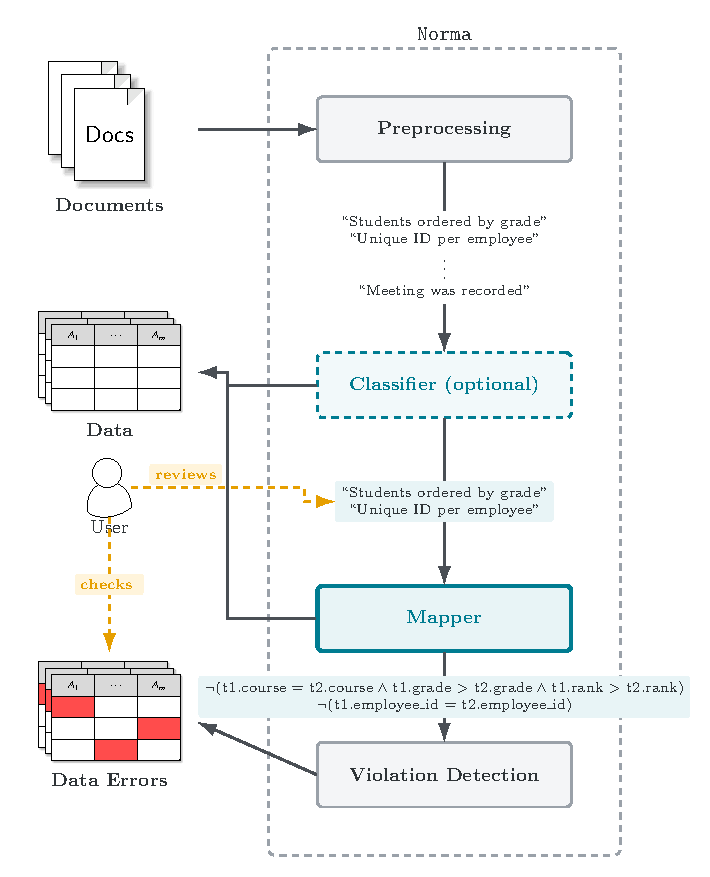
\includegraphics[width=\columnwidth]{diagramas/pipeline_norma.pdf}
%\caption{The \system\ pipeline.}
\vspace{-10pt}
\caption{Overview of the \system\ pipeline. Blue components represent the novel contributions presented in this paper.}
\label{fig:pipeline}
\vspace{-10pt}
\end{figure}

\smallskip\noindent\textbf{Preprocessing.}
We start from documents (e.g., PDF files) and produce a normalized text representation.
This step can be noisy\subs{, as headers and footers often leak into the body, line breaks split tokens, footnotes disrupt reading order, and lists get flattened into fragments that hinder sentence boundary detection.}{ (e.g., leaked headers, split tokens, and flattened lists).} Since our goal is Text-to-Constraints 	rather than document conversion, we treat preprocessing as input preparation and do not focus on it in this work. We run an automated pipeline covering text extraction,	dehyphenation, whitespace normalization, and sentence segmentation, followed by minimal manual cleanup.


\smallskip\noindent\textbf{Constraint classifier.}
Given the sentences from preprocessing, a lightweight classifier can optionally identify those that likely express checkable constraints, filtering out content that \subs{surely has nothing to do with}{is clearly unrelated to} data quality constraints.  Since constraints missed at this stage cannot be recovered downstream, we prioritize recall at this stage. False positives can still be ruled out by the mapper\subs{, which applies a more expressive classification strategy internally}{ (which we define next)}. \add{The classifier only labels the given sentences and never generates text, so it preserves the link between each sentence and its constraint.} When no classifier is used, all sentences are passed directly to the mapper. A user can optionally be involved at this stage, reviewing and correcting the set of classified sentences before proceeding to mapping. We describe the classifier details in Section~\ref{sec:classifier}.


\smallskip\noindent\textbf{Constraint mapper.}
The mapper is the central and most complex component of \system. It takes each sentence, optionally pre-filtered by the classifier, and produces a denial constraint grounded in the dataset schema.\rem{ Some mapper implementations have an internal classification step that uses schema-based information to decide whether a sentence yields a valid constraint before attempting to construct one.}
The mapper must interpret natural language, align it with schema elements, and synthesize a constraint with correct violation semantics. Outputs that fail syntactic validation are rejected, and sentences that yield no valid constraint are excluded from the final output. We describe the different mapper implementations in detail in Section~\ref{sec:mapper}.


\smallskip\noindent\textbf{Violation detection.}
Each constraint is validated by compiling it into a SQL violation query and executing it on the target relation (Section~\ref{sec:mapper:sql}), and it is linked back to the sentence that produced it. \system\ returns the violating tuples to the user for further inspection. DC violation detection is a well-studied problem, with specialized systems available for large-scale consistency checks~\cite{facet2021,liu2024rapidash,youri2024}. \add{We compile DCs into SQL because the queries run on any engine that holds the data and also serve the data-based checks of the mapper; specialized engines can replace this step for larger workloads.}


 
\section{Constraint Classification}
\label{sec:classifier}
Given the segment set $\mathcal{S}$ extracted from a regulatory document, the constraint classifier aims at identifying the subset $\mathcal{S}_c \subseteq \mathcal{S}$ of segments that state data quality constraints. A segment is a positive example if it expresses a condition that the data is expected to satisfy and that can be 
validated against a dataset. Many segments only define terms, describe procedures, or provide context. Constraint-related segments appear less often, and many segments that sound like rules are still too vague to test with data. 


For ease of exposition, we treat each segment as a single sentence from now on, unless stated otherwise.

\begin{example}[Restaurant inspections]
\label{ex:classification}
The NYC Department of Health publishes restaurant inspection results, 
including scores and letter grades,\footnote{Dataset available at 
\url{https://data.cityofnewyork.us/Health/DOHMH-New-York-City-Restaurant-Inspection-Results/43nn-pn8j}. See Section~\ref{sec:experiments} for details.} alongside a document 
describing the grading and inspection regulations.\footnote{Available at 
\url{https://www.nyc.gov/site/doh/services/restaurant-grades.page}.} 
Table~\ref{tab:sentence-types} shows sample sentences from these 
regulations. The first two sentences state data quality rules that can be validated when the dataset contains the needed information. The first connects score ranges to letter grades and can be checked by comparing the score and grade fields. The second constraint defines inspection frequency per establishment and can be checked when establishment identifiers and inspection dates are available. The last two are not data quality rules: one is too underspecified to test because it does not define which inspections yield grades, and the other describes user permissions rather than a condition on the data.
\begin{table}[ht]
\centering
\small
\begin{tabular}{p{0.75\columnwidth}c}
\toprule
\textbf{Sentence} & \textbf{Constraint?} \\
\midrule
A score of 0--13 results in a grade of A. & Yes \\
Every food service establishment is scheduled for at least one inspection per year. & Yes \\
Only certain inspections result in a grade. & No \\
Consumers may check an establishment's inspection history. & No \\
\bottomrule
\end{tabular}
\caption{Constraint vs. non-constraint sample sentences from NYC restaurant inspection regulations.}
\label{tab:sentence-types}
\end{table}
\qed
\end{example}
%\vspace{-1cm}

%At this stage, we prioritize recall over precision: missed rules cannot be recovered downstream, while false positives can still be filtered by the constraint mapper. \system\ treats the classifier as a replaceable module that outputs binary labels or confidence scores. This modularity allows implementations to be swapped for cost, accuracy, or domain considerations. \system\ currently supports two types of classifier implementations.


%% use this if we include the SLM classifier
%At this stage, we prioritize recall over precision: missed rules cannot be recovered downstream, while false positives can still be filtered by the constraint mapper. \system\ treats the classifier as a replaceable module that outputs binary labels or confidence scores. This modularity allows implementations to be swapped for cost, accuracy, or domain considerations. \system\ currently supports two types of classifier implementations: \emph{LLM-based prompting} and \emph{fine-tuned encoders}. The LLM is more flexible and can incorporate schema and data samples at inference time, generalizing better out-of-domain but incurring API costs. The fine-tuned model is faster and cheaper but depends on training data diversity. Section~\ref{sec:experiments} quantifies these trade-offs.
    
%At this stage, we prioritize recall over precision: missed rules cannot be recovered downstream, while false positives can still be filtered by the constraint mapper. 
\system\ implements the classifier via \emph{LLM-based prompting}, which can incorporate schema and data samples at inference time and generalizes across domains without requiring labeled training data.

%\smallskip\noindent\textbf{LLM-Based Classification}
%\subsection{LLM-Based Classification}
\subsection*{Constraint Classification by Example}
%\label{sec:classifier:llm}
%We prompt large language models to label each sentence as stating a data quality rule or not. Figure~\ref{fig:classifyprompt} shows the prompt structure (full prompts are in the supplementary material). We use prompt variants that optionally include generic template examples and schema context (table description, columns, and sample tuples). We require structured output and parse responses with regular expressions; if parsing fails after retries, we default to non-constraint. Section~\ref{sec:experiments} evaluates closed- and open-weight models under these variants.

We ask a large language model to label each sentence as either stating a data quality rule or not. Figure~\ref{fig:classifyprompt} shows how the prompt is generally structured. 
%In our setting, some prompt variations include generic template examples and schema context, such as table descriptions, columns, and sample tuples.
Our design is inspired by few-shot in-context learning~\cite{brown2020language}, where a model is guided by a small number of task examples provided in the input context. In our case, these examples are generic and independent of the target domain, serving to guide the model’s structured reasoning over candidate constraints.
%In our setting, labeled sentence templates, schema information, and sample tuples guide the model's labeling decisions across a large and heterogeneous sentence space. 
The model returns one label per numbered sentence through a JSON schema. Malformed outputs are retried, then the sentences of the batch are classified one at a time, and a sentence that still has no valid label is marked as non-constraint. Section~\ref{sec:experiments} compares closed- and open-weight models using these prompt versions.


\begin{figure}[!ht]
\centering
\footnotesize
\begin{tabularx}{\linewidth}{p{0.15\linewidth}X}
\toprule
\textbf{Task Definition} &
\hlc[neutralbg]{For each sentence, decide whether it states a DATA QUALITY CONSTRAINT that can be validated from the dataset when the required fields are available.}\\
\midrule

\textbf{Rule Types} &
%\hlc[neutralbg]{YES: includes:} \newline
\hlc[yesbg]{Required/non-null field; Allowed or forbidden values; Numeric bounds; Conditional requirements; Cross-row consistency; Determinacy; Temporal constraints; \ldots} \\
\midrule

\textbf{Exclusions} &
%\hlc[neutralbg]{NO: includes:} \newline
\hlc[nobg]{Headings, titles, citations; Definitions or descriptions; Procedures or human decisions; Statements not testable from the dataset; \ldots} \\
\midrule

\textbf{Notes} &
%\hlc[neutralbg]{Clarifications for edge cases:} \newline
\hlc[neutralbg]{Modal verbs (``may'', ``should'') do not disqualify a sentence; what matters is whether it describes a data condition or verifiable property; \ldots} \\
\midrule

\textbf{Examples} \newline \textit{(optional)} &
\hlc[neutralbg]{YES:} \newline
\hlc[yesbg]{``Field X is required.''} \newline
\hlc[yesbg]{``Two rows with the same Key must not disagree on Field H.''} \newline
\hlc[yesbg]{\ldots} \newline
\hlc[neutralbg]{NO:} \newline
\hlc[nobg]{``Field X represents the total amount.''} \newline
\hlc[nobg]{\ldots} \\
\midrule

\textbf{Context} \newline \textit{(optional)} &
%\hlc[neutralbg]{Table:} \hlc[contextbg]{[\textsf{Table Description}]} \newline
\hlc[neutralbg]{Table Schema:} \hlc[contextbg]{[\textsf{Column Names / Types}]} \newline
\hlc[neutralbg]{Table Sample Rows:} \hlc[contextbg]{[\textsf{Example Tuples}]} \\
\midrule

\textbf{Input} &
\hlc[neutralbg]{Sentences:} \newline
\hlc[neutralbg]{[\textsf{Numbered List of Sentences}]} \newline
\hlc[neutralbg]{Return one YES/NO label per sentence number} \\
\bottomrule
\end{tabularx}

\vspace{-0.3cm}
\caption{Constraint classification prompt structure (simplified).
Colors indicate: \csquare{yesbg}\,positive label clues, \csquare{nobg}\,negative label clues, \csquare{contextbg}\,data context, and \csquare{neutralbg}\,instructions.}
\vspace{-0.3cm}
\label{fig:classifyprompt}
\end{figure}


%\smallskip\noindent\textbf{Prompt structure.} Following standard practice in prompt-based text classification~\cite{sun2023textclassification}, we include a task definition, category descriptors, and optional labeled examples. 
%We find this strategies important, as constraint classification presents two challenges. First, the positive class is rare and heterogeneous, with many syntactic forms. We enumerate rule types to reduce false negatives; otherwise, models may miss constraints such as functional dependencies, where a key (or key-like attribute set) determines another attribute (e.g., two rows with the same key must agree on a field), and other cross-row consistency conditions.
%Second, the negative class is easily confused with constraints. Definitions, procedures, and contextual statements often use similar wording, refer to data-related terms, or include keywords that suggest a requirement. We list exclusions and add notes for common edge cases.

\smallskip\noindent\textbf{Prompt structure.}
Following standard practice in prompt-based text classification~\cite{sun2023textclassification}, we include a task definition, category descriptors, and examples.
These elements are essential because constraint classification presents two main challenges.
The first challenge is that the positive class is rare and spans \subs{ }{}many syntactic forms.
To reduce false negatives, we enumerate rule types that the model should treat as constraints. Otherwise, it may miss cases such as functional dependencies that might use specific language. 
%We also include examples of cross-row consistency conditions. 
The second challenge is that non-constraint sentences can be easily mistaken for constraints. Definitions, procedures, and contextual statements often use similar wording, mention data-related concepts, or contain keywords that suggest a requirement. To reduce this confusion, we explicitly add notes on exclusions and edge cases.

\smallskip\noindent\textbf{Examples.} Our approach follows a \subs{ }{}few-shot prompting strategy~\cite{brown2020language}, using generic templates that remain fixed across datasets, rather than domain-specific examples. As a result, the prompt remains portable without requiring labeled data.

%To further illustrate this, in Section~\ref{sec:experiments}, we evaluate the impact of examples on recall.



\smallskip\noindent\textbf{Table Context.}
We evaluated multiple prompt variants. 
Some ask the classifier to decide from the sentence alone whether it expresses a checkable constraint.
Others also provide table context, including table and column information and sample tuples. Without access to the schema, the classifier may
produce false positives for sentences that cannot be checked against the
available fields. Schema context helps reject such cases and, therefore, mainly improves precision. 
However, it also increases prompt length and can make predictions sensitive to the particular sample tuples provided.

\smallskip\noindent\textbf{Batch processing.}
To reduce API overhead, \system\ classifies sentences in batches, concatenating 
multiple sentences into a single prompt using numeric indices and parsing one 
label per index from the response. We use moderate batch sizes (up to 10 sentences 
per prompt)\rem{, as larger batches increase prompt length and the risk of truncated 
outputs and parsing errors}. Malformed responses trigger a retry\rem{; if the model 
still fails, we fall back to processing the remaining sentences individually}.











%\subsection{Fine-Tuned Classifier}
%\label{sec:classifier:finetuned}
%
%Prompting an LLM for each sentence can be expensive for long documents. As a lower-cost alternative, we finetune a pretrained encoder to screen sentences before the mapping stage. Constraint classification can be viewed as a binary text classification problem: given a sentence, predict whether it states a data quality rule.
%
%\smallskip\noindent\textbf{Pretrained encoders for text classification.}
%Text classification with pretrained language models is well studied~\cite{plmClassification2025}. We follow the standard finetuning approach based on BERT~\cite{devlin-etal-2019-bert}: a pretrained encoder produces a sentence representation, and a lightweight classification head predicts the binary label. Finetuning pretrained encoders is a common transfer learning approach for natural language classification tasks and typically performs well even with limited labeled data~\cite{gururangan-etal-2020-dont}. Several encoder variants are available, including general-domain BERT-style models and domain-specific models such as Legal-BERT~\cite{chalkidis-etal-2020-legal} for legal text. We evaluate multiple variants in Section~\ref{sec:experiments}.
%
%In this implementation, we use sentence-only input to keep the classifier fast and compatible with smaller encoder models that have a limited maximum input length (in tokens). Joint text-and-schema encoding is possible for table-related tasks~\cite{TURL2022}, but we leave schema-aware encoders for this type of classifier as future work. Schema context is still supported in the LLM-based classifier.
%
%
%\smallskip\noindent\textbf{Adapting to the constraint domain.}
%Pretrained encoders learn from broad textual corpora, but text on data rules represents a narrower linguistic domain with specific vocabulary and structure. Prior work shows that adapting language models to the target domain can improve downstream performance~\cite{gururangan-etal-2020-dont}. However, collecting training data for the data quality domain is difficult: the boundary between constraint and non-constraint sentences is subtle and requires high expertise, making large-scale annotation expensive. To address this, we propose generating synthetic training data using an LLM guided by explicit instructions that describe the constraint domain.
%
%\smallskip\noindent\textbf{Training data generation.}
%Recent work shows that LLM-generated data can approach real-world data for training text classifiers when the task is objective and well-defined~\cite{li-etal-2023-synthetic}. However, models trained on synthetic data can overfit to surface patterns if the generated examples lack diversity~\cite{data_augmentation2020}. We propose two complementary strategies to address this.
%
%\emph{Paraphrase augmentation} takes labeled sentences from other datasets and prompts the LLM to generate variants that preserve meaning while changing wording and structure. For each seed sentence, we generate multiple paraphrases, increasing lexical diversity within each constraint type and helping the classifier generalize beyond specific phrasings.
%
%\emph{Schema-grounded synthesis} prompts the LLM with the target schema (column names and sample tuples), labeled examples from other datasets, and a list of common rule patterns (required fields, allowed values, numeric bounds, cross-row consistency, determinacy).
%The LLM generates new sentences that reference actual column names from the target schema. This increases coverage across constraint types relevant to the target dataset. We apply the same setup to synthesize non-constraint sentences, targeting definitions, procedures, and contextual statements that cover difficult negatives.
%
%
%Note that we exclude labeled sentences from the target document from training, and schema information is used only to guide the LLM during generation. This makes the approach portable as a fine-tuned classifier can be trained for any new dataset without manual annotation.
%
%
%%Together, paraphrases increase variation within observed rule types, while schema-grounded synthesis increases coverage across rule patterns tied to the schema.
%
%
%\smallskip\noindent\textbf{Training.}
%Constraint sentences are rare in regulatory documents, creating class imbalance that biases the model toward predicting non-constraint. We oversample constraint sentences and apply focal loss~\cite{focalLoss2020}, which down-weights easy negatives and focuses training on difficult examples such as non-constraints that resemble rules.
%Since lower encoder layers capture general linguistic patterns and upper layers are task-specific~\cite{rogers-etal-2020-primer}, we use layerwise learning rate decay to preserve pretrained knowledge in lower layers while allowing upper layers to adapt. Training details are in the supplementary material.
%
%
%\smallskip\noindent\textbf{Threshold selection.}
%The classifier outputs a probability $P(\text{constraint} \mid s)$ for each sentence. A threshold of 0.5 maximizes accuracy, but since missed constraints cannot be recovered downstream, we tune the threshold on a validation set to achieve recall of at least 0.85 while maximizing precision.
 
\section{Constraint Mapping}
\label{sec:mapper}

Let $\mathcal{S}$ denote the sentences passed to the mapper, either all preprocessed sentences or the subset retained by the classifier. For each $s_i \in \mathcal{S}$, the mapper returns a denial constraint (DC) $\varphi_i = \neg(p_1 \land \cdots \land p_\ell)$ over the dataset schema, or no output if $s_i$ does not express a constraint or cannot be linked to the schema.

Recall from Section~\ref{sec:problem} that DC predicates can take several forms, including comparisons between an attribute and a constant (e.g., \texttt{t.A = c}), between two attributes of the same tuple (e.g., \texttt{t.A > t.B}), or between attributes across tuples (e.g., \texttt{t1.A = t2.A}), as well as null checks and membership tests over permitted values.
The mapping task is therefore to interpret a sentence, identify the relevant schema elements, select the predicates on those elements that capture the constraint intuition, and produce an executable \emph{violation condition}. In this sense, it is related to Text-to-SQL~\cite{yu2018spider}, as both tasks aim to connect a natural language segment to schema-aware logical expressions. One key difference is that Text-to-SQL typically retrieves satisfying records, whereas our target is a conjunction of predicates that identify a constraint violation.

\begin{example}[Mapping to DC predicates]
\label{ex:mapping}
Consider the sentence ``A score of 0--13 results in a grade of A'' from the NYC restaurant inspection regulations. This sentence states that scores in the range 0--13 must be associated with grade A. The corresponding violation condition is:
\[
\texttt{t.score} \geq \texttt{0} \land \texttt{t.score} \leq \texttt{13} \land \texttt{t.grade} \neq \texttt{`A'}
\]
Any tuple satisfying all three predicates violates the rule. \qed
\end{example}

Mapping regulatory text to DCs is challenging because the same rule may be expressed in many different ways, often with implicit references to schema elements, literals, or tuple relationships. 
We therefore rely on LLM-based mappers, motivated by their strong performance on related semantic parsing tasks such as Text-to-SQL~\cite{llmTEXT2SQLSurvey2025}. However, unrestricted LLM generation is unreliable in our setting\subs{, it is known that LLMs  can hallucinate}{: LLMs are known to hallucinate} column names and use unsupported operators~\cite{dail2025,llmTEXT2SQLSurvey2025,DBLP:conf/dexa/DociniAO25}. 
We also observed that LLMs tend to output predicates describing valid states rather than violations, so we introduce hints toward violations in the prompt.

To make mapping tractable and reliable, our design follows two principles. First, we derive a \emph{predicate space} from the dataset schema and use it as a controlled vocabulary. The mapper must either select predicates from this space or instantiate typed placeholders within predefined predicate templates. This reduces the search space and prevents ill-formed outputs. Second, the mapper is biased toward \emph{precision}. Incorrect mapping can generate false violations and corrupt downstream checks, whereas an unmapped sentence can still be marked for manual inspection.

We implement two mapper variations that share the same predicate space but differ in how they use it. The \emph{single-prompt mapper} (Section~\ref{sec:mapper:llm}) performs the full mapping in a single LLM call, while the \emph{multi-step mapper} (Section~\ref{sec:mapper:multistep}) decomposes the task into focused LLM calls interleaved with deterministic checks. Both produce DCs that are compiled into SQL violation queries (Section~\ref{sec:mapper:sql}).


\subsection{Predicate Space}
\label{sec:mapper:predicate-space}

Traditional DC discovery operates over a \emph{predicate space}, that is, the set of predicates allowed to appear in candidate constraints~\cite{chu2013discovering,Pena2019DiscoveryDC}. Because discovery methods enumerate and validate combinations of predicates, this space is kept small, which limits expressiveness~\cite{chu2013discovering}.

Our setting requires a richer predicate space. Regulatory text frequently refers to \subs{explicit literals, enumerations, ranges, nullability conditions, and string formats that are not covered by traditional DC discovery spaces.}{enumerations, ranges, string formats, and arithmetic conditions. Comparisons with constants and null checks are expressible as DCs, but discovery spaces rarely include set membership, patterns, or arithmetic, because each extension multiplies the candidates to enumerate.} We therefore extend the predicate space with typed predicate templates that can be instantiated with literals extracted from text. Importantly, \system\ does not enumerate \subs{candidates DC  over}{candidate DCs over} this larger space. Instead, it uses the space as a controlled vocabulary for mapping, which avoids candidate explosion while preserving syntactic validity.

\smallskip\noindent\textbf{Predicate templates.}
We derive a finite set of predicates and predicate templates from the schema, while the data instance is used to support specific instantiations and validation steps. We consider the following categories:
\begin{enumerate}
    \item \textbf{Cross-tuple predicates} compare attributes across two tuples (e.g., \texttt{t1.A = t2.A}, \texttt{t1.A > t2.B}). We allow $\{=,\neq\}$ for type-compatible attributes and additionally $\{<,\leq,>,\geq\}$ for numeric attributes.
    \item \textbf{Same-tuple predicates} compare two attributes within one tuple (e.g., \texttt{t1.A $\leq$ t1.B}), capturing intra-tuple rules.
    \item \textbf{Null predicates} (\texttt{t1.A IS NULL}, \texttt{t1.A IS NOT NULL}) capture requiredness and conditional missingness constraints.
    \item \textbf{Attribute--constant predicates} compare an attribute to a constant $c$ (e.g., \texttt{t1.A = c}, \texttt{t1.A $\geq$ c}).
    \item \textbf{Pattern predicates} encode string-format and substring conditions (e.g., \texttt{t1.A LIKE p}).
    \item \textbf{Set predicates} encode membership in small enumerations (e.g., \texttt{t1.A IN C}).
    \item \textbf{Arithmetic predicates} compare an arithmetic expression over numeric attributes of the same tuple with an attribute or a constant (e.g., \texttt{t1.A $\geq$ c * t1.B}), when the schema enables arithmetic for those attributes.
\end{enumerate}
For categories 4--7, the mapper instantiates the placeholders $c$, $p$, or $C$ using literals extracted from the sentence.
\add{\smallskip\noindent\textbf{Coverage and limits.} Across our six datasets, 487 of the 490 predicates of the gold DCs belong to this space. The three exceptions, on HMDA Checks, compare an integer-encoded date with an arithmetic expression over the reporting year. The categories exclude aggregation and arithmetic over dates or sequences of records, so rules over counts or inspection histories require derived attributes, such as the days until the next inspection in Restaurant (Section~\ref{sec:datasets}).}


\smallskip\noindent\textbf{Predicate restrictions.}
To avoid semantically uninformative or implausible predicates, we adopt a filtering principle from DC discovery~\cite{chu2013discovering}. Order predicates are generated only for numeric attributes. Cross-tuple and same-tuple predicates are generated only for type-compatible pairs and are further pruned using observed value overlap, helping eliminate comparisons between unrelated columns.
\rem{Nonetheless, our extensions with predicate templates, constants, patterns, and sets expand the predicate space from the dozens common in DC discovery to several hundred in some datasets. This space is impractical for traditional data profiling, where the enumeration cost grows exponentially with the number of predicates. In our approach, the larger predicate space remains practical because we use it only as a constrained target language for mapping, not as a search space for enumerating combinations.}


\smallskip\noindent\textbf{Schema-driven, on-demand predicate space.}
Materializing the full space does not scale to wide schemas: with arithmetic and
code-set templates, the space of a 135-column table reaches hundreds of thousands
of templates, most of which are irrelevant to any given sentence. \system\
therefore stores only a \emph{schema description} and generates predicates on
demand. For each column, the description records its type, the comparison and
arithmetic operators it admits, its domain values when it has at most a few
distinct values, and a short natural-language description. Descriptions are
written once, offline, by an LLM from a deterministic profile of the data\rem{ (type,
null rate, distinct values, ranges, frequent values, format patterns, and observed
code--label pairs)}; when an official data dictionary is available, its
definitions are merged into the description of the corresponding columns (we do
this for HMDAZ, using the FFIEC field definitions). At mapping time, once the
relevant columns of a sentence are selected, the predicates of the categories
above are generated only for those columns, under the same restrictions. For a
fixed instance and fixed options, the generated set equals the full space
restricted to the selected columns, so the controlled vocabulary is unchanged;
only its materialization is deferred.

\subsection{Single-Prompt Mapper}
\label{sec:mapper:llm}

The single-prompt mapper performs the full mapping in a single LLM call. 
We design the prompt around three elements: the schema and predicate space as a controlled vocabulary, a small set of examples covering the main constraint patterns, and predicate specifications to guide the model in understanding and mapping violation conditions. Given an input sentence, the model returns either \subs{a list of predicates drawn from the predicate space}{a list of rules over the retrieved columns and their predicates} or \texttt{null}. 
Figure~\ref{fig:mapprompt} summarizes the prompt structure.
\subs{In the current version, the}{The} prompt is restricted to the columns retrieved for
the sentences of each batch (three sentences per call): columns are ranked by
the embedding similarity between the sentence and the column name and
description\rem{ (semantic retrieval)}, and the prompt carries the description and
domain values of each retrieved column\rem{ (column context)} together with the
predicates generated for them. The model must also state, for each sentence,
the condition under which a tuple violates the rule (\texttt{violated\_when})
before writing the DC, which makes the violation form explicit.\rem{ Rules that
reference unknown columns or compare a column with a constant of the wrong type
are returned to the model once, with the error message.}





\begin{figure}[!ht]
\centering
\footnotesize
\begin{tabularx}{\linewidth}{p{0.2\linewidth}X}
\toprule
\textbf{Definition} &
\hlc[neutralbg]{A denial constraint (DC) is a conjunction of predicates 
that \emph{cannot} all hold simultaneously in a dataset. DC predicates 
must encode \emph{violations} of data quality rules, not valid states.} \\
\midrule
\textbf{Violation Form} &
\hlc[neutralbg]{``must be X'' $\Rightarrow$ \texttt{!= X};
``must not be X'' $\Rightarrow$ \texttt{= X};} \\
\midrule
\textbf{Cross-Tuple} &
\hlc[neutralbg]{Signals such as ``same \ldots'', ``repeated'', or ``consecutive'' introduce \texttt{t1}, \texttt{t2}, and a join predicate on the shared key.} \\
\midrule
\textbf{Context} &
\hlc[contextbg]{Table schema + top-$k$ frequent values per column.} \newline
\hlc[contextbg]{List of possible predicates (predicate space).} \\
\midrule
\textbf{Examples} &
\hlc[yesbg]{``Value must be at least 100''}
$\Rightarrow$ \texttt{["t1.value < 100"]} \newline
\hlc[yesbg]{``Same ID must share status''}
$\Rightarrow$ \texttt{["t1.id = t2.id", "t1.status != t2.status"]} \newline
\hlc[nobg]{``The system performs well''}
$\Rightarrow$ \texttt{null} \\
\midrule
\textbf{Output} &
\hlc[neutralbg]{Array of length $n$, one entry per input sentence; \texttt{null} for non-constraints. Predicates must come from the predicate space.} \\
\bottomrule
\end{tabularx}
\caption{Prompt structure for the single-prompt mapper. Examples are 
representative, as the full prompt covers threshold, set-membership, 
field-comparison, null, cross-tuple, and non-constraint cases. The colors represent: 
\csquare{contextbg}\,Data context; \csquare{yesbg}\,constraint example; 
\csquare{nobg}\,non-constraint; \csquare{neutralbg}\, instructions.}
\label{fig:mapprompt}
\end{figure}

\smallskip\noindent\textbf{Violation form.}
Without explicit guidance, LLMs generally tend to output predicates describing 
\emph{satisfying} tuples rather than \emph{violating} ones. Since 
regulatory sentences typically describe what must hold, the mapper must 
find predicates expressing a violation condition---as in Example~\ref{ex:mapping}, 
where the correct output is \texttt{grade $\neq$ `A'}, not \texttt{grade $=$ `A'}. 
We make this criterion explicit in the prompt through a small set of examples.



\smallskip\noindent\textbf{Cross-tuple constraints.}
Some rules address relationships between records rather than conditions 
within a single record. In these cases, the mapper must introduce two 
tuple aliases and a join predicate on the shared identifier. %---producing, for instance, \texttt{t1.id = t2.id} alongside the distinguishing predicate. 
Including cues such as ``for the same'' in the prompt
already suffices for the model to generalize reliably to the variety of phrasings in which such predicates appear.
\add{The target remains a DC with at most two tuple variables and universal violation semantics: a single violating pair suffices. Rules that must hold only for most pairs, or that compare distances between values, such as differential dependencies, would require counting or tolerance semantics and are outside our scope.}



\smallskip\noindent\textbf{Literal grounding.}
Many constraints require grounding numeric thresholds, strings, or small 
enumerations. A recurring failure is to produce literals in the wrong 
format or casing. To mitigate this, we include in the prompt \subs{the top-$k$ 
frequent values per column as a domain context}{the description and the domain values of each retrieved column}, which anchors 
literals to the dataset representation\add{ (e.g., a label such as \texttt{'Secured by a first lien'} rather than a paraphrase)}.\rem{ In practice, we found that fewer than ten 
samples per column usually suffice for the model to capture the relevant patterns.}

The mapper returns \subs{at most one DC per sentence}{for each sentence a list of independent rules, whose violations are united (Section~\ref{sec:mapper:sql})}. If the sentence is not mappable, it returns \texttt{null}. We parse the output and validate every predicate against the schema: it must reference existing columns, use operators admitted by their types, compare them with constants of the right type, and have no uninstantiated placeholders. Membership in the generated predicate space is not enforced for this mapper; we report it instead (out-of-space predicates). Malformed outputs are retried a fixed number of times, and invalid rules are returned once to the model with the error. If all attempts fail, the sentence produces no constraint. To prevent incorrect mappings from affecting downstream checks, we intentionally keep this stage conservative.


\smallskip\noindent\textbf{Batch processing.}
As in the classifier (Section~\ref{sec:classifier}), we support batch processing by concatenating multiple indexed sentences into one prompt and returning one output per index. 
%We use the same moderate batch sizes and fallback strategy.

\subsection{Multi-Step Mapper}
\label{sec:mapper:multistep}
The single-prompt mapper needs to parse several subtasks in one call: schema linking, predicate selection, literal linking, and  violation form. In this setting, errors in early steps might sometimes propagate. For example, a wrong column choice may break predicate selection, a hallucinated literal yields a syntactically valid but semantically meaningless constraint, and a non-constraint sentence triggers an unnecessary mapping attempt. Recent work in Text-to-SQL shows that decomposing semantic parsing into multiple stages, especially separating schema linking from later query building decisions, often improves accuracy~\cite{DBLP:conf/dexa/DociniAO25,redsql2025,dail2025,llmTEXT2SQLSurvey2025}. 


We propose a multi-step mapper that breaks down mapping into several LLM calls, with deterministic checks in between.
The process uses four LLM calls, where each call receives the output from the previous step. Sentences that cannot be mapped are
removed before constraint construction. After construction, data-driven checks
eliminate constraints that have incorrect literals\add{ or implausible violation sets}.
\add{Each stage isolates one decision that the single-prompt mapper must make jointly (columns, DC structure, whether the sentence is a rule, and literals), so the stages trade additional calls for smaller decisions that can each be validated. In our experiments, this decomposition keeps the mapper usable with backbones whose single-prompt outputs fail, and the rule filter rejects most non-constraint sentences without a construction call (Section~\ref{sec:experiments}). A finer ablation that removes or reorders individual stages is left for future work.}

Figure~\ref{fig:multistep-pipeline} illustrates the control flow of our multi-step mapper and
Figure~\ref{fig:multistepprompt} provides a summary of its prompts in each step.

%, andFigure~\ref{fig:multistep-trace} illustrates an execution trace.



\begin{figure}[ht!]
    \centering
    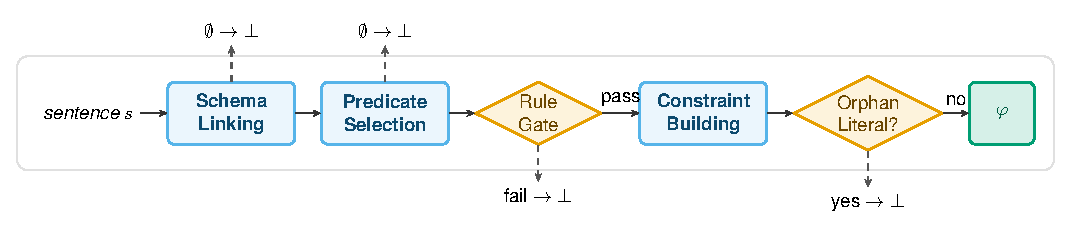
\includegraphics[width=\columnwidth]{diagramas/multistep_diagram.pdf}
    \caption{Multi-step mapper control flow.}
    \label{fig:multistep-pipeline}
\end{figure}



\begin{figure}[ht!]
\centering
\footnotesize
\begin{tabularx}{\linewidth}{p{0.13\linewidth}p{0.28\linewidth}X}
\toprule
\textbf{Step} & \textbf{Context} & \textbf{Task} \\
\midrule

\textbf{Schema} &
\hlc[contextbg]{Full schema, column profiles, predicate space} &
\hlc[neutralbg]{Identify all columns relevant to $s$: direct mentions, synonyms, and derived concepts.}
\hlc[nobg]{Abort if no concept maps to any column with defined predicates.} \\

\midrule

\textbf{Predicates} &
\hlc[contextbg]{$\hookrightarrow$ Columns from Schema step} \newline
\hlc[contextbg]{Predicate space restricted to those columns} \newline
\hlc[contextbg]{Column profiles} &
\hlc[neutralbg]{Select predicates and predicate templates from the restricted predicate space and identify the constraint pattern for $s$ (value mapping, temporal bound, functional dependency, required field, or conditional rule).}
\hlc[nobg]{Abort if no predicate or predicate template fits.} \\

\midrule

\textbf{Rule filter} &
\hlc[contextbg]{$\hookrightarrow$ Columns and predicates from Predicates step} &
\hlc[neutralbg]{Decide whether $s$ expresses a specific, data quality rule verifiable from column values alone.} \newline
\hlc[nobg]{Reject: process descriptions, permissions, vague quantifiers, physical conditions.} \newline
\hlc[yesbg]{Accept: value mappings, temporal bounds, functional dependencies, required fields, conditional rules.} \\

\midrule

\textbf{Construction} &
\hlc[contextbg]{$\hookrightarrow$ Predicates and predicate templates from Predicates step} \newline
\hlc[contextbg]{Column profiles} &
\hlc[neutralbg]{Substitute predicate placeholders with literals from $s$ and return the constraint in violation form: a conjunction of predicates that must not hold simultaneously.} \\

\bottomrule
\end{tabularx}
\caption{Prompt structure of the multi-step mapper. Context narrows progressively. The rule filter runs after predicate selection but before construction, avoiding unnecessary LLM calls on non-rules.
\csquare{contextbg}\,input context (variable per step);
\csquare{yesbg}\,accept signal;
\csquare{nobg}\,abort\,/\,reject signal;
\csquare{neutralbg}\,fixed instruction.}
\label{fig:multistepprompt}
\end{figure}

\smallskip\noindent\textbf{Schema linking.}
This step identifies the columns relevant to the sentence, including implicit 
references and derived concepts.\rem{ We prompt the model to return the set of columns relevant for the sentence, since operating over a smaller, relevant subset reduces the risk of incorrect predicate selection in the later step.} If no column with defined predicates can be aligned to any concept in the sentence, we reject the sentence for mapping.

\smallskip\noindent\textbf{Predicate selection.} The mapper uses only columns retained by schema linking. Given the column names, profiles, and restricted predicate spaces, it selects predicates and predicate templates (requiring literals) that together form the DC pattern. \rem{We separate column selection from predicate selection to address distinct subproblems: schema linking determines which attributes are relevant to a sentence, while predicate selection determines how those attributes are combined into a denial-constraint structure. This decomposition reduces the DC structural search space and helps avoid predicates that, while individually plausible, do not compose into a valid constraint. }This \subs{design aligns}{separation aligns} with prior results in text-to-SQL, where having a dedicated structural parsing step has been shown to improve accuracy~\cite{resdsql2023}.

\smallskip\noindent\textbf{Rule filter.}
This step determines whether the sentence can be mapped to a DC under the schema-grounded interpretation obtained so far. Unlike the classifier in Section~\ref{sec:classifier}, the rule filter has access to the candidate columns and predicates selected for the sentence. This improves the semantic reliability of the decision, since many sentences that appear rule-like in isolation \subs{may fail to support a coherent executable constraint once their concepts are grounded in the schema and tied to candidate predicates}{support no executable constraint once grounded in the schema}. %We therefore place the filter after predicate selection, where this evidence is available. %, but before construction, to avoid unnecessary literal grounding for sentences that should still be rejected.
%
%\smallskip\noindent\textbf{Constraint building.}
%This step builds the final DC by instantiating the selected predicate templates with literals extracted from the sentence. Since the candidate columns and predicate forms have already been fixed, construction no longer needs to search the full predicate space. Instead, it resolves the value-level details required by the selected templates, such as numeric thresholds, categorical values, ranges, patterns, and small enumerations. We use the column profiles with sample values to align these literals with the dataset's representation. The goal is to preserve details such as casing, abbreviations, and formatting used in the data and map that to the term in the sentence.. 
%The output is produced as a set of predicates representing  in violation form. Restricting this step to grounded instances of previously selected templates reduces the risk of hallucinated predicates and ill-formed constraints~\cite{pourreza2023din,picard2021}.

\smallskip\noindent\textbf{Constraint building.}
This step instantiates the selected predicate templates with the literals needed to form the final DC.\rem{ At this point, the candidate columns and predicate types have already been fixed, so the task is no longer to explore the full predicate space, but to realize a small set of grounded predicate instances.} The model resolves value-level details such as numeric thresholds, categorical constants, intervals, string patterns, and short enumerations, and aligns them with the dataset representation using column profiles and sample values. \rem{This grounding is important because the text and the data often use different representations. A sentence may describe a concept in natural language, while the table records it as an abbreviation, code, or differently formatted value. }The output is a set of predicates in violation form, which are then assembled into the final DC. Framing this stage as grounded instantiation rather than open-ended generation substantially narrows the construction problem and makes unsupported predicates and malformed expressions less likely~\cite{pourreza2023din,picard2021,lin-etal-2020-bridging}.


\smallskip\noindent\textbf{Post-construction checks.}
After constructing a candidate DC, \subs{both sentence-level mappers apply}{the multi-step mapper applies} a set of validation checks to ensure that the generated constraints are both executable and semantically plausible. First, we verify the structural validity of the DC: each predicate must belong to the predicate space, reference valid schema columns, use type-compatible operators, and contain no uninstantiated placeholders. Next, we apply a data-based grounding check for unsupported literals. For each predicate with literals involving equality, string inequality, \texttt{LIKE}, or set membership, we issue an existence query against the dataset. If no tuple can satisfy the predicate, we refer to it as an \emph{orphan predicate}, \subs{i.e.,,}{i.e.,} a predicate that is syntactically valid but unsupported by the data instance. Any constraint containing \subs{a orphan predicate is disregard for validation}{an orphan predicate is discarded}, although it may be retained for documentation purposes. \add{Finally, we execute the DC and discard it when more than 90\% of the tuples take part in a violation: a DC that flags almost every tuple most likely encodes the valid state rather than its violation. The single-prompt mapper applies only the schema validation described in Section~\ref{sec:mapper:llm}.} 
Numeric bounds and \texttt{null} predicates are excluded from this check because their validity is structural rather than value-based.
If parsing fails, the mapper retries a small fixed number of times; if all attempts fail, no constraint is returned.

%\begin{figure}[t]
%    \centering
%    \includegraphics[width=\columnwidth]{diagramas/multistep_diagram_trace.pdf}
%    \caption{Example execution trace of the multi-step mapper.}
%    \label{fig:multistep-trace}
%\end{figure}


\subsection{From Denial Constraints to SQL}
\label{sec:mapper:sql}

Every DC produced by \system\ is compiled into a SQL \emph{violation query}, which is used for the data-based checks of the mappers, for violation detection, and for evaluation. The compilation is deterministic, but it has to settle several questions that the DC formalism leaves open when it meets real data.

\smallskip\noindent\textbf{Rule structure.}
For each sentence, the mapper returns a list of independent rules. Each rule is a tree of \texttt{AND}/\texttt{OR} nodes over the predicate forms of Section~\ref{sec:problem}\rem{, extended with arithmetic over numeric attributes of the same tuple}. A rule whose body contains disjunctions is equivalent to a set of DCs, one per disjunct of its disjunctive normal form, so it remains a denial constraint.\rem{ It lets a single rule keep the alternative branches of one requirement, such as the thresholds of a regulation that differ by lien type.} Independent rules of the same sentence are compiled separately, and their violations are united.

\smallskip\noindent\textbf{Compilation.}
A rule with one tuple variable becomes a selection over the relation that returns the identifiers of the violating tuples. A rule with two tuple variables becomes a self-join with the condition $t_1.\mathit{tid} \neq t_2.\mathit{tid}$.\rem{ Predicates are rendered recursively.} Membership and pattern predicates map to \texttt{IN} and \texttt{LIKE}, division is guarded against zero divisors, and literals are written in a canonical form (e.g., \texttt{1} for \texttt{1.0}). The self-join condition must not be replaced by an ordering such as $t_1.\mathit{tid} < t_2.\mathit{tid}$, a common way to avoid reporting a pair twice. That shortcut is only correct for symmetric DCs, such as functional dependencies. For an asymmetric DC, such as the ordering rule of Example~\ref{ex:intro}, it misses every violating pair whose witnesses appear in the opposite order: on SISU, the ordering rule flags 61 applications with $\neq$ but only 9 with $<$. Since violations are reported at the tuple level, enumerating both orders does not inflate the counts.

\smallskip\noindent\textbf{Types and missing values.}
Published data rarely matches its declared schema. Numeric fields contain codes such as \texttt{NA} or \texttt{Exempt}\rem{, and some files are best read as text to avoid lossy type inference}. We therefore read the data as text, type each column with the schema, and compare numeric attributes through safe casts (\texttt{TRY\_CAST}), which turn malformed values into \texttt{NULL} rather than aborting the query. Under SQL's three-valued logic, a predicate over \texttt{NULL} is unknown, so the tuple is not reported.\rem{ This is the intended behavior for a missing salary in an ordering rule.} However, it means that requiredness must be stated explicitly with \texttt{IS NULL}, and that a disequality such as \texttt{loan\_type != 1} silently skips tuples without a loan type. The mapper prompts illustrate requiredness with \texttt{IS NULL} predicates and ask for missing values to be written that way\rem{, and the evaluation unifies code and label literals only when the data confirms that they select the same tuples (Section~\mbox{\ref{sec:metrics}})}.

\smallskip\noindent\textbf{Execution.}
Queries run on DuckDB over the published files.\rem{ Single-tuple queries scale linearly, but a pair DC whose join attributes have few distinct values can produce a quadratic number of bindings.}\rem{ A model-generated rule that joins only on a state column, for instance, may produce billions of pairs.} Each query therefore runs under a memory budget, a time limit, and a cap on the result size. A query that exceeds them is reported as an execution error, never as a constraint without violations.

\smallskip\noindent\textbf{Bridging text and data.}
Most of the difficulty lies before compilation, in the inferences that the mapper must make so that the compiled query checks what the text means. Table~\ref{tab:sql-examples} shows real constraints from our datasets. On Tax, the comparative ``lower salary cannot have higher tax rate'' becomes an asymmetric pair DC. On SISU, ``selected in only one of their options'' requires the mapper to identify the student by the national ID rather than by the exam registration number, a choice that the text leaves implicit. On HMDA Checks, monetary amounts are recorded in thousands, so ``\$1,000 (\$1 million)'' becomes \texttt{loan\_amount >= 1000}, and ``five times the income'' becomes an arithmetic predicate. On HMDAZ, the regulation compares the annual percentage rate with the average prime offer rate, a difference that the register stores as \texttt{rate\_spread}. The trigger also combines coverage conditions, three alternative thresholds, and label columns whose values (e.g., \texttt{'Secured by a first lien'}) must match the data verbatim.\rem{ On Restaurant, the yearly-inspection requirement can only be checked through a derived attribute (\texttt{days\_to\_next\_inspection}), since our DCs do not aggregate over inspection sequences.} Each of these decisions changes the violating tuples, which is why violation detection is reported next to structural extraction in our evaluation.

\begin{table*}[t]
  \centering
  \footnotesize
  \setlength{\tabcolsep}{4pt}
  \begin{tabular}{>{\raggedright\arraybackslash}p{1.6cm}>{\raggedright\arraybackslash}p{4.6cm}>{\raggedright\arraybackslash}p{9.0cm}r}
    \toprule
    \textbf{Dataset} & \textbf{Sentence (abridged)} & \textbf{Violation condition in the compiled query (\texttt{WHERE} clause, casts omitted)} & \textbf{Viol.} \\
    \midrule
    Restaurant & A score of 0--13 results in a grade of A. & \texttt{t1.score >= 0 AND t1.score <= 13 AND t1.grade != 'A'} & 402 \\
    Tax & Within the same state, a person with lower salary cannot have higher tax rate. & \texttt{t1.tid <> t2.tid AND t1.state = t2.state AND t1.salary < t2.salary AND t1.rate > t2.rate} & 363 \\
    SISU & The student will be selected in only one of their options.$^{\dagger}$ & \texttt{t1.tid <> t2.tid AND t1.cpf = t2.cpf AND t1.edicao = t2.edicao AND t1.ano = t2.ano AND t1.etapa = t2.etapa AND t1.opcao != t2.opcao AND t1.aprovado = 'S' AND t2.aprovado = 'S'} & 149 \\
    HMDA Checks & If loan amount and income are $>0$ and the loan amount is $\geq$ \$1,000 (\$1 million), then loan amount should be $<$ 5 times the income. & \texttt{t1.loan\_amount > 0 AND t1.applicant\_income > 0 AND t1.loan\_amount >= 1000 AND t1.loan\_amount >= (5 * t1.applicant\_income)} & 600 \\
    HMDA Checks & If purchaser type = 1 or 3, then loan type should = 1. & \texttt{t1.purchaser\_type IN (1, 3) AND t1.loan\_type != 1} & 441 \\
    HMDAZ & A high-cost mortgage is a consumer credit transaction secured by the consumer's principal dwelling in which the APR exceeds the APOR by more than (A) 6.5 points for a first lien, (B) 8.5 points for a first lien on personal property under \$50,000, or (C) 8.5 points for a subordinate lien. & \texttt{t1.business\_or\_commercial\_purpose = 2 AND t1.occupancy\_type\_name = 'Principal residence' AND t1.reverse\_mortgage\_name = 'Not a reverse mortgage' AND t1.hoepa\_status\_name = 'Not a HOEPA loan' AND ((t1.lien\_status\_name = 'Secured by a first lien' AND (t1.manufactured\_home\_secured\_property\_type != 2 OR t1.loan\_amount >= 50000) AND t1.rate\_spread > 6.5) OR (t1.lien\_status\_name = 'Secured by a first lien' AND t1.manufactured\_home\_secured\_property\_type = 2 AND t1.loan\_amount < 50000 AND t1.rate\_spread > 8.5) OR (t1.lien\_status\_name = 'Secured by a subordinate lien' AND t1.rate\_spread > 8.5))} & 4 \\
    \bottomrule
  \end{tabular}
  \caption{Gold constraints of our datasets compiled into violation queries, with the number of violating tuples (HMDA: first 1M rows). Each query selects the identifiers of the tuples bound to \texttt{t1} (and \texttt{t2}) that satisfy the condition; numeric attributes are compared through \texttt{TRY\_CAST}. $^{\dagger}$Translated from Portuguese.}
  \label{tab:sql-examples}
\end{table*}

{\ifReview\color{blue}\fi
\subsection{Methodological Contributions}
\label{sec:mapper:novelty}

Table~\ref{tab:novelty} delineates which components of \system\ build on Text-to-SQL practice and which are specific to mapping normative text to constraints. Prompts implement individual decisions, but replacing a prompt changes neither the vocabulary, the violation form, nor the checks that every constraint must pass.

\begin{table}[!ht]
  \centering
  \footnotesize\ifReview\color{blue}\fi
  \setlength{\tabcolsep}{3pt}
  \begin{tabular}{>{\raggedright\arraybackslash}p{2.1cm}>{\raggedright\arraybackslash}p{1.3cm}>{\raggedright\arraybackslash}p{4.6cm}}
    \toprule
    \textbf{Component} & \textbf{Origin} & \textbf{What is specific to \system} \\
    \midrule
    Schema linking & Adapted~\cite{resdsql2023,pourreza2023din} & Over a schema description with column descriptions and domain values (Section~\ref{sec:mapper:predicate-space}). \\
    Staged decomposition & Adapted~\cite{pourreza2023din} & A rule filter decides whether the text is a checkable rule at all; every Text-to-SQL question has an answer. \\
    Predicate space & New & Typed templates derived from the schema and generated on demand for the selected columns. \\
    Violation form & New & The output is the condition that must never hold (a DC), a canonical target instead of a query. \\
    Data-grounded checks & New & Orphan literals and the share of violating tuples are checked on the instance. \\
    Compilation & New & Pair, type, and \texttt{NULL} semantics of the violation queries (Section~\ref{sec:mapper:sql}). \\
    Evaluation & New & Equivalence-aware extraction, execution equivalence, and per-rule metrics (Section~\ref{sec:metrics}). \\
    \bottomrule
  \end{tabular}
  \caption{Components of \system\ adapted from Text-to-SQL and components specific to Text-to-Constraints.}
  \label{tab:novelty}
\end{table}
}



%\begin{algorithm}[ht!]
%\caption{Multi-Step Mapper}
%\label{alg:multistep}
%\small
%\begin{algorithmic}[1]
%\Input{sentence $s$, predicate space $\mathcal{P}$, dataset $\mathcal{D}$}
%\Output{denial constraint $\varphi$, or $\bot$}
%\State $C \gets \Call{SchemaLinking}{s, \mathcal{P}}$
%\State \textbf{abort if} $C = \emptyset$
%\State $P, \pi \gets \Call{PredicateSelection}{s, C, \mathcal{P}|_C}$
%\State \textbf{abort if} $P = \emptyset$
%\State \textbf{abort if} $\neg\Call{FilterNonRules}{s,C,P,\pi}$
%\State $\varphi \gets \Call{BuildConstraint}{s, C, P}$
%\State \textbf{abort if} $\varphi = \emptyset$
%\State \textbf{abort if} $\Call{DeadLiteral}{\varphi, \mathcal{D}}$
%\State $cnt \gets \Call{Execute}{\varphi, \mathcal{D}}$
%\State \Return $\varphi$ \textbf{if} $\Call{CheckViolations}{\varphi, cnt}$ \textbf{else} $\bot$
%\end{algorithmic}
%\end{algorithm} 



\section{Experimental Evaluation}
\label{sec:experiments}

We implemented a prototype of \system\ and evaluated it on several datasets prepared for the \emph{Text-to-Constraints} setting. Our evaluation is organized around the following questions.
\begin{itemize}[leftmargin=0.5cm]
    \item \textbf{RQ1: Constraint-sentence classification.} How accurately can \system\ identify which sentences in a normative document express data constraints?

    \item \textbf{RQ2: Mapping quality.} Given constraint-relevant text, how accurately can \system\ map it to executable denial constraints and  how well do these constraints capture the corresponding data violations?

    \item \textbf{RQ3: Impact of implementation choices.} How do different classifier and mapper implementations, LLM backends, and prompt variants affect extraction quality and robustness?

    \item \textbf{RQ4: Comparison with baselines.} How does \system\ compare with data profiling and Text-to-SQL baselines on constraint extraction and violation detection?
\end{itemize}

\subsection{Datasets}
\label{sec:datasets}

%No benchmark currently exists for the \emph{Text-to-Constraints} problem.
%We prepared four datasets for our experiments. Two are based on real-world regulatory documents paired with corresponding tabular datasets, and two are derived from datasets widely used in data quality and profiling research, for which the target constraints are already known. For the real-world datasets, we manually annotated the constraints expressed in the source text. For the derived datasets, we generated natural-language descriptions of the known constraints, as described below. When a constraint had no natural violations in the data, we injected a few violating records so that every constraint could be evaluated under the violation-based metrics of Section~\ref{sec:metrics}. 
%Table~\ref{tab:datasets} summarizes the datasets.


We evaluate \system\ on six datasets: four based on real-world regulatory documents paired with corresponding tabular datasets, and two derived from benchmark datasets commonly used in data quality and profiling research. A summary of these datasets is provided in Table~\ref{tab:datasets}, including the number of rows and columns, the number of sentences in the source text, the number of annotated constraints, and the number of tuples violating at least one constraint. \add{For every dataset, the authors labeled each sentence and wrote its gold DC in violation form over the released schema; sentences not checkable on the released attributes are non-constraints. No sentence occurs twice, and near-identical sentences (similarity $\geq 0.9$) are templated statements that differ in one attribute or literal (13 pairs in SISU, 32 in HMDA Checks, at most two elsewhere), never sharing a gold DC.}



\begin{table}[ht]
  \centering
\small
%  \resizebox{\columnwidth}{!}{%
  \begin{tabular}{lrrrrr}
    \toprule
    \textbf{Dataset} & \textbf{\#Rows} & \textbf{\#Cols} & \textbf{Sent.} & \textbf{Const.} & \textbf{Viol.} \\
    \midrule
    Hospital & 1k & 17 & 109 & 15 & 834 \\
    Restaurant & 128k & 21 & 33 & 7 & 52,311 \\
    SISU & 102k & 56 & 42 & 17 & 533 \\
    Tax & 100k & 15 & 126 & 6 & 468 \\
    HMDAZ$^{\dagger}$ & 1M & 135 & 17 & 9 & 209 \\
    HMDA Checks$^{\dagger}$ & 1M & 81 & 158 & 92 & 986,491 \\
    \bottomrule
  \end{tabular}%
  %}% resizebox
    \caption{Dataset statistics. $^{\dagger}$First 1M rows of the public file (15.1M and 4.8M rows); \emph{Const.} counts sentences mapped to a non-null gold DC.}
  \label{tab:datasets}
\end{table}

\smallskip\noindent\textbf{SISU.}
As discussed in Section~\ref{sec:intro}, the SISU dataset contains admission
records from Brazil's centralized university selection system. We manually
annotated three sections of \textit{Portaria Normativa No.~21/2012} covering student
registration, candidate classification and selection, and waitlist procedures.
The resulting constraints span \subs{nullability checks, functional dependencies,
ordering constraints, and conditional selection rules.}{11 nullability checks, a functional dependency, an order dependency (Example~\ref{ex:intro}), a conditional functional dependency (a student is selected in at most one option), and three conditional DCs over one or two tuples (e.g., a student selected in the first option cannot be selected in the second).} Many have violations in
the released data, suggesting inconsistencies between the published records and
the regulatory requirements expressed in the text.


\smallskip\noindent\textbf{Restaurant.}
As introduced in Example~\ref{ex:classification}, this dataset contains
restaurant inspection records published by the Department of Health and Mental
Hygiene of New York. We annotated the NYC food service operator
inspection guide, focusing on the grading and closure sections, which present
constraints on score-to-grade mappings, inspection frequency, grade posting
timing, and closure conditions. Most have natural violations and can be
grounded directly to existing fields. For the one constraints that reasons over
inspection sequences, we added one derived column that tracks the days until the next inspection. We leave to future work how \system\ can guide or automate such dataset
transformations more systematically.


\smallskip\noindent\textbf{Tax and Hospital.}
Both datasets have been widely used in data profiling and denial-constraint
research since the seminal work of Chu et al.~\cite{chu2013discovering}. For
Tax, we extracted the constraint descriptions from the original
paper~\cite{chu2013discovering}. For Hospital, we used the data and constraints from
a well-known cleaning system~\cite{holoclean}. Because their constraints are available in
formal form, we first generated natural-language descriptions with an LLM. For
both datasets, we then prompted an LLM to generate additional non-constraint
sentences around each rule, mimicking a regulatory document that interleaves
binding rules with other prose. The prompt receives the schema and is
instructed to use schema terminology, making sentence classification more
challenging. To avoid circularity between data generation and evaluation, we used Claude~4.5 Sonnet, a model not
evaluated in any \system\ configuration. \add{These two datasets nevertheless form a controlled setting: their constraints come from prior papers and their sentences from an LLM that may share priors with the evaluated backbones, which likely makes them easier than real regulatory text. SISU, Restaurant, and the HMDA datasets, which pair real regulatory text with real data, are the more reliable signal.}




\smallskip\noindent\textbf{HMDAZ and HMDA Checks.}
Both datasets use public loan-level records released under the Home Mortgage
Disclosure Act (HMDA)\rem{ and are, by far, the largest in our evaluation}; we use the
first 1M rows of each file. \emph{HMDAZ} pairs the 2018 loan application
register (135 columns, including the code and label versions of each
categorical field) with Sections 1026.32, 1026.35, and 1026.43 of Regulation~Z,
which define high-cost (HOEPA) and higher-priced mortgages, the limitations
that apply to them\rem{ (e.g., balloon payments, negative amortization, prepayment
penalties)}, and the ability-to-repay requirements. Sentences are verbatim from
the regulation, and gold DCs keep the coverage conditions of each trigger\rem{ (e.g.,
a loan is high-cost only if it is a closed-end, principal-residence loan)}.
Scope-only text, or text whose outcome is not observable in the data, is
annotated with a \texttt{null} constraint. \emph{HMDA Checks} pairs the 2014
register (81 columns) with the 2014 HMDA edit specification published by the
FFIEC: one entry per edit, with the edit test verbatim; edits that cannot be
checked on a single record (aggregate, transmittal-sheet, or external-reference
edits) are \texttt{null}. These datasets stress three aspects that the \subs{original
four do not}{other datasets lack}: wide schemas whose relevant column is often named after a code
rather than the concept in the text, rules that compare columns with each other
or through arithmetic\rem{ (e.g., loan amount versus five times the income)}, and a
highly concentrated violation distribution (Section~\ref{sec:metrics}).

\subsection{Baselines}
\label{sec:baselines}

Since no prior system addresses the Text-to-Constraints task directly, we compare \system\ against the two closest paradigms: DC discovery from data alone and Text-to-SQL.


\smallskip\noindent\textbf{Data profiling.}
We use the DC discovery algorithms from~\cite{Pena2022FastDC}, running both exact and approximate denial-constraint discovery. Exact discovery returns only constraints that hold on the data with no violations. As a result, it is not suitable for our violation-based evaluation, which aims to recover rules that may be violated in the released dataset. We therefore focus on approximate DC discovery as the main profiling baseline. Approximate DCs allow a small fraction of violating tuple pairs, controlled by a threshold $\varepsilon$, and can therefore recover rules even when the data is not fully clean. \add{Since FDs and order dependencies with at most two tuples are special cases of DCs, approximate DC discovery over the same attributes subsumes their discovery, and we do not run separate FD or OD algorithms. Conditional variants require predicates with constants, which DC discovery supports only for a restricted set of values; a comparison with dedicated CFD discovery is left for future work.}

Because discovery can return many DCs, we rank them using the standard
criterion from prior work~\cite{chu2013discovering}, which combines coverage
and succinctness, with succinctness measured as the inverse of the number of
symbols in the DC. We run exact discovery and $\varepsilon \in \{0.001, 0.005, 0.01, 0.05, 0.1\}$, evaluate top-$k \in \{5, 10, 20, 50, 100\}$, and report, for each metric, the best result across these settings, following standard practice in prior work.

These baselines do not scale to our largest schemas. In particular, they
cannot process SISU, Restaurant, or the HMDA datasets with all columns present.
For those datasets, we therefore restrict the input to the subset of columns that appear
in the gold constraints, giving the profiling baselines the best possible
setting under their scalability limits, and run discovery on a seeded sample of
100k of the 1M HMDA rows. On HMDA Checks (39 columns), no configuration finished:
runs timed out (6\,h with 100k rows, 2\,h with 50k) or exhausted a 12\,GB heap
even with samples of 20k and 10k rows.


\smallskip\noindent\textbf{Text-to-SQL.}
We use XiYan-SQL~\cite{XiYanSQL}, a state-of-the-art generative text-to-SQL
framework. We adapt it to our setting by prompting it, for each sentence, to
return a SQL query that identifies the tuples violating the described
constraint, or \texttt{NULL} if the sentence does not express a checkable data
constraint. Under this formulation, XiYan-SQL acts jointly as a constraint
classifier and mapper, making it directly comparable to \system\ across all
evaluation dimensions. We use the 32B model with three seeds and report the mean.


\subsection{Evaluation Metrics}
\label{sec:metrics}

Text-to-Constraints requires solving three related problems: identify
text that expresses constraints, translate those into a formal
representation, and identify the data violations implied by those constraints.
We therefore evaluate systems along three complementary dimensions:
\textit{Constraint Classification}, \textit{Constraint Extraction}, and
\textit{Violation Detection}. This is similar in spirit to Text-to-SQL evaluation, where
execution-based evaluation complements structural matching because exact form
alone does not fully capture correctness~\cite{zhong-etal-2020-semantic}. Because \system\ and the
baselines in Section~\ref{sec:baselines} differ in what they produce, not all
dimensions apply to every method.

\smallskip\noindent\textbf{Constraint Classification.}
This dimension measures whether a system correctly identifies which sentences
in a document express constraints. We report precision, recall, and F$_1$
over all sentences. This dimension applies to sentence-level variants of
\system\ and to the Text-to-SQL baseline. It does not apply to data profiling
baselines, which operate on data rather than text.

\smallskip\noindent\textbf{Constraint Extraction.}
This dimension measures how accurately systems translate text into denial
constraints. We compare predicted and ground-truth constraints by
predicate-set match (i.e., exact matching over the set of predicates), and report precision, recall, and F$_1$. For \system\
and the data profiling baselines, the predicate set is read directly from the
predicted denial constraint. For Text-to-SQL, we extract predicates from the
\texttt{WHERE} clause of the generated query. A correlated \texttt{EXISTS} is read as a pair DC; a query with no DC
reading, e.g., with aggregation or \texttt{CASE}, counts as a correct extraction
if it returns exactly the violations of the gold DC of its sentence, so that
equivalent SQL formulations are not penalized. For data profiling, discovered constraints are
matched directly against the ground-truth set.

\smallskip\noindent\textbf{Violation Detection.}
This dimension measures whether the constraints produced by a system, when
executed on the dataset, identify the same tuples as the
ground-truth constraints. Because a denial constraint may involve either a
single tuple or a pair of tuples, we evaluate violations at the tuple level by
counting tuples that participate in at least one violation. We execute all predicted
constraints and all ground-truth constraints on the dataset, then compare the
resulting violation sets using precision, recall, and F$_1$. This dimension
applies to all \system\ variants and all baselines.


\smallskip\noindent\textbf{Complementary mapping metrics.}
Exact predicate-set matching penalizes logically equivalent rewritings, and the
tuple-level aggregate can be dominated by a single rule. We therefore report
four complementary measures for the mappers. (i)~\emph{Equivalence-aware
extraction} (CE$_{\equiv}$) compares DCs after a logical normal form \subs{that expands
\texttt{IN}/\texttt{NOT IN}, orients and sorts operands, flattens and
distributes \texttt{AND}/\texttt{OR}, and removes absorbed terms}{(e.g., \texttt{IN} as a disjunction, sorted operands, distributed \texttt{AND}/\texttt{OR})}; in addition,
\subs{an equality literal on a code column and the equality literal on its label
column (e.g., \texttt{hoepa\_status = 1} and \texttt{hoepa\_status\_name = 'High-cost
mortgage'}) are unified only when the data confirms that both select exactly the
same tuples. Code--label pairs are discovered in the data, not from column
names.}{literals on a code column and on its label column (e.g., \texttt{hoepa\_status = 1} and \texttt{hoepa\_status\_name = 'High-cost mortgage'}) are unified only when the data confirms that they select the same tuples.} (ii)~\emph{Execution equivalence} is the fraction of gold rules with at
least one violation whose predicted DC flags exactly the same tuples.
(iii)~\emph{Per-rule violation F$_1$} averages, over gold sentences, the F$_1$
between the tuples flagged by the gold and the predicted DC, so that every rule
weighs the same. (iv)~\emph{Violation concentration} is the share of the
gold-violating tuples flagged by the single largest gold rule\rem{; it is a property
of the dataset, not of the method}. We also count predicted DCs whose SQL fails
to execute, instead of treating them as producing no violation.


\subsection{Implementation and Execution Settings}
\label{sec:implementation}

\system\ is implemented in Python, with DuckDB as the query execution backend.
All LLM calls are issued through OpenRouter with strict JSON-schema structured
outputs. We evaluate six backbones: GPT-6 Luna, DeepSeek-V4-Flash, Mistral Large 4,
Qwen3.8-2.4T-A95B, GPT-6 Sol, and Claude Sonnet 5.5.\rem{ Before the runs, every
backbone passed a health check of the classifier, both single-prompt output
schemas, and each Multi-Step schema.} Two candidates were replaced: Kimi K2.6,
which repeatedly emitted whitespace until the token limit under strict
JSON-schema decoding, and MiniMax-M3, which returned empty single-prompt outputs
in the experiments (Section~\ref{sec:constraintextraction}). Each configuration is executed once, with a cap of 32k
output tokens per call. Unless stated otherwise, \system\ uses the schema-driven
predicate space of Section~\ref{sec:mapper:predicate-space} with on-demand predicate
generation, and the single-prompt mapper uses semantic column retrieval and
column context (Section~\ref{sec:mapper:llm}). Constraints are executed on the
full datasets (first 1M rows for HMDA) with DuckDB. \system\ experiments were
executed on a Linux workstation with an Intel Core i7-7700HQ CPU and 16\,GB of
memory, as were the DC discovery baselines (Java 21). The XiYan-SQL
baseline, which requires GPU inference, was executed on an
NVIDIA A100 SXM GPU (80\,GB VRAM). The baselines are scored by the same
evaluator, data, and query limits as \system.

%\smallskip\noindent\textbf{Efficiency} reports total wall-clock runtime and, for
%LLM-based approaches, estimated API cost per dataset, enabling analysis of the
%quality-cost trade-off across \textsc{Norma} configurations and baselines.



% \subsection{Implementation and Execution Settings}
% \label{sec:implementation}

% \system\ is implemented in Python, using DuckDB as the query execution
% backend. LLM calls are
% issued via the OpenAI API (GPT-5, GPT-5-mini), the Mistral API
% (Mistral-Small, Mistral-Large), the Groq API (Llama-3.3-70B), and the Qwen API (Qwen3-32B).
% All \system\ experiments and DC discovery baselines were executed on
% a MacBook Pro with an Apple M1 chip and 16\,GB of unified memory.
% Baselines requiring GPU inference were executed on a cloud server
% equipped with an NVIDIA A100 SXM GPU (80\,GB VRAM, 125\,GB RAM,
% 16\,vCPUs).
 
\subsection{Classifier Performance}
\label{sec:constraintdetection}

Our first experiment evaluates how model and prompt design affect the accuracy of constraint classification. Starting from the prompt in Figure~\ref{fig:classifyprompt} (Section~\ref{sec:classifier}), we derive four
variants by enabling or disabling \emph{constraint examples} and
\emph{table context}: \emph{No Context}, \emph{Table Context},
\emph{Examples}, and \emph{Examples + Table Context}. We evaluate all four variants across six LLMs and all six datasets. Figure~\ref{fig:classifier-results} summarizes the results. Because sentences missed at this stage cannot be recovered later by the mapper, we require a recall of at least 0.90 on every dataset when selecting a default configuration (red dashed line).

\begin{figure}[!ht]
    \centering
    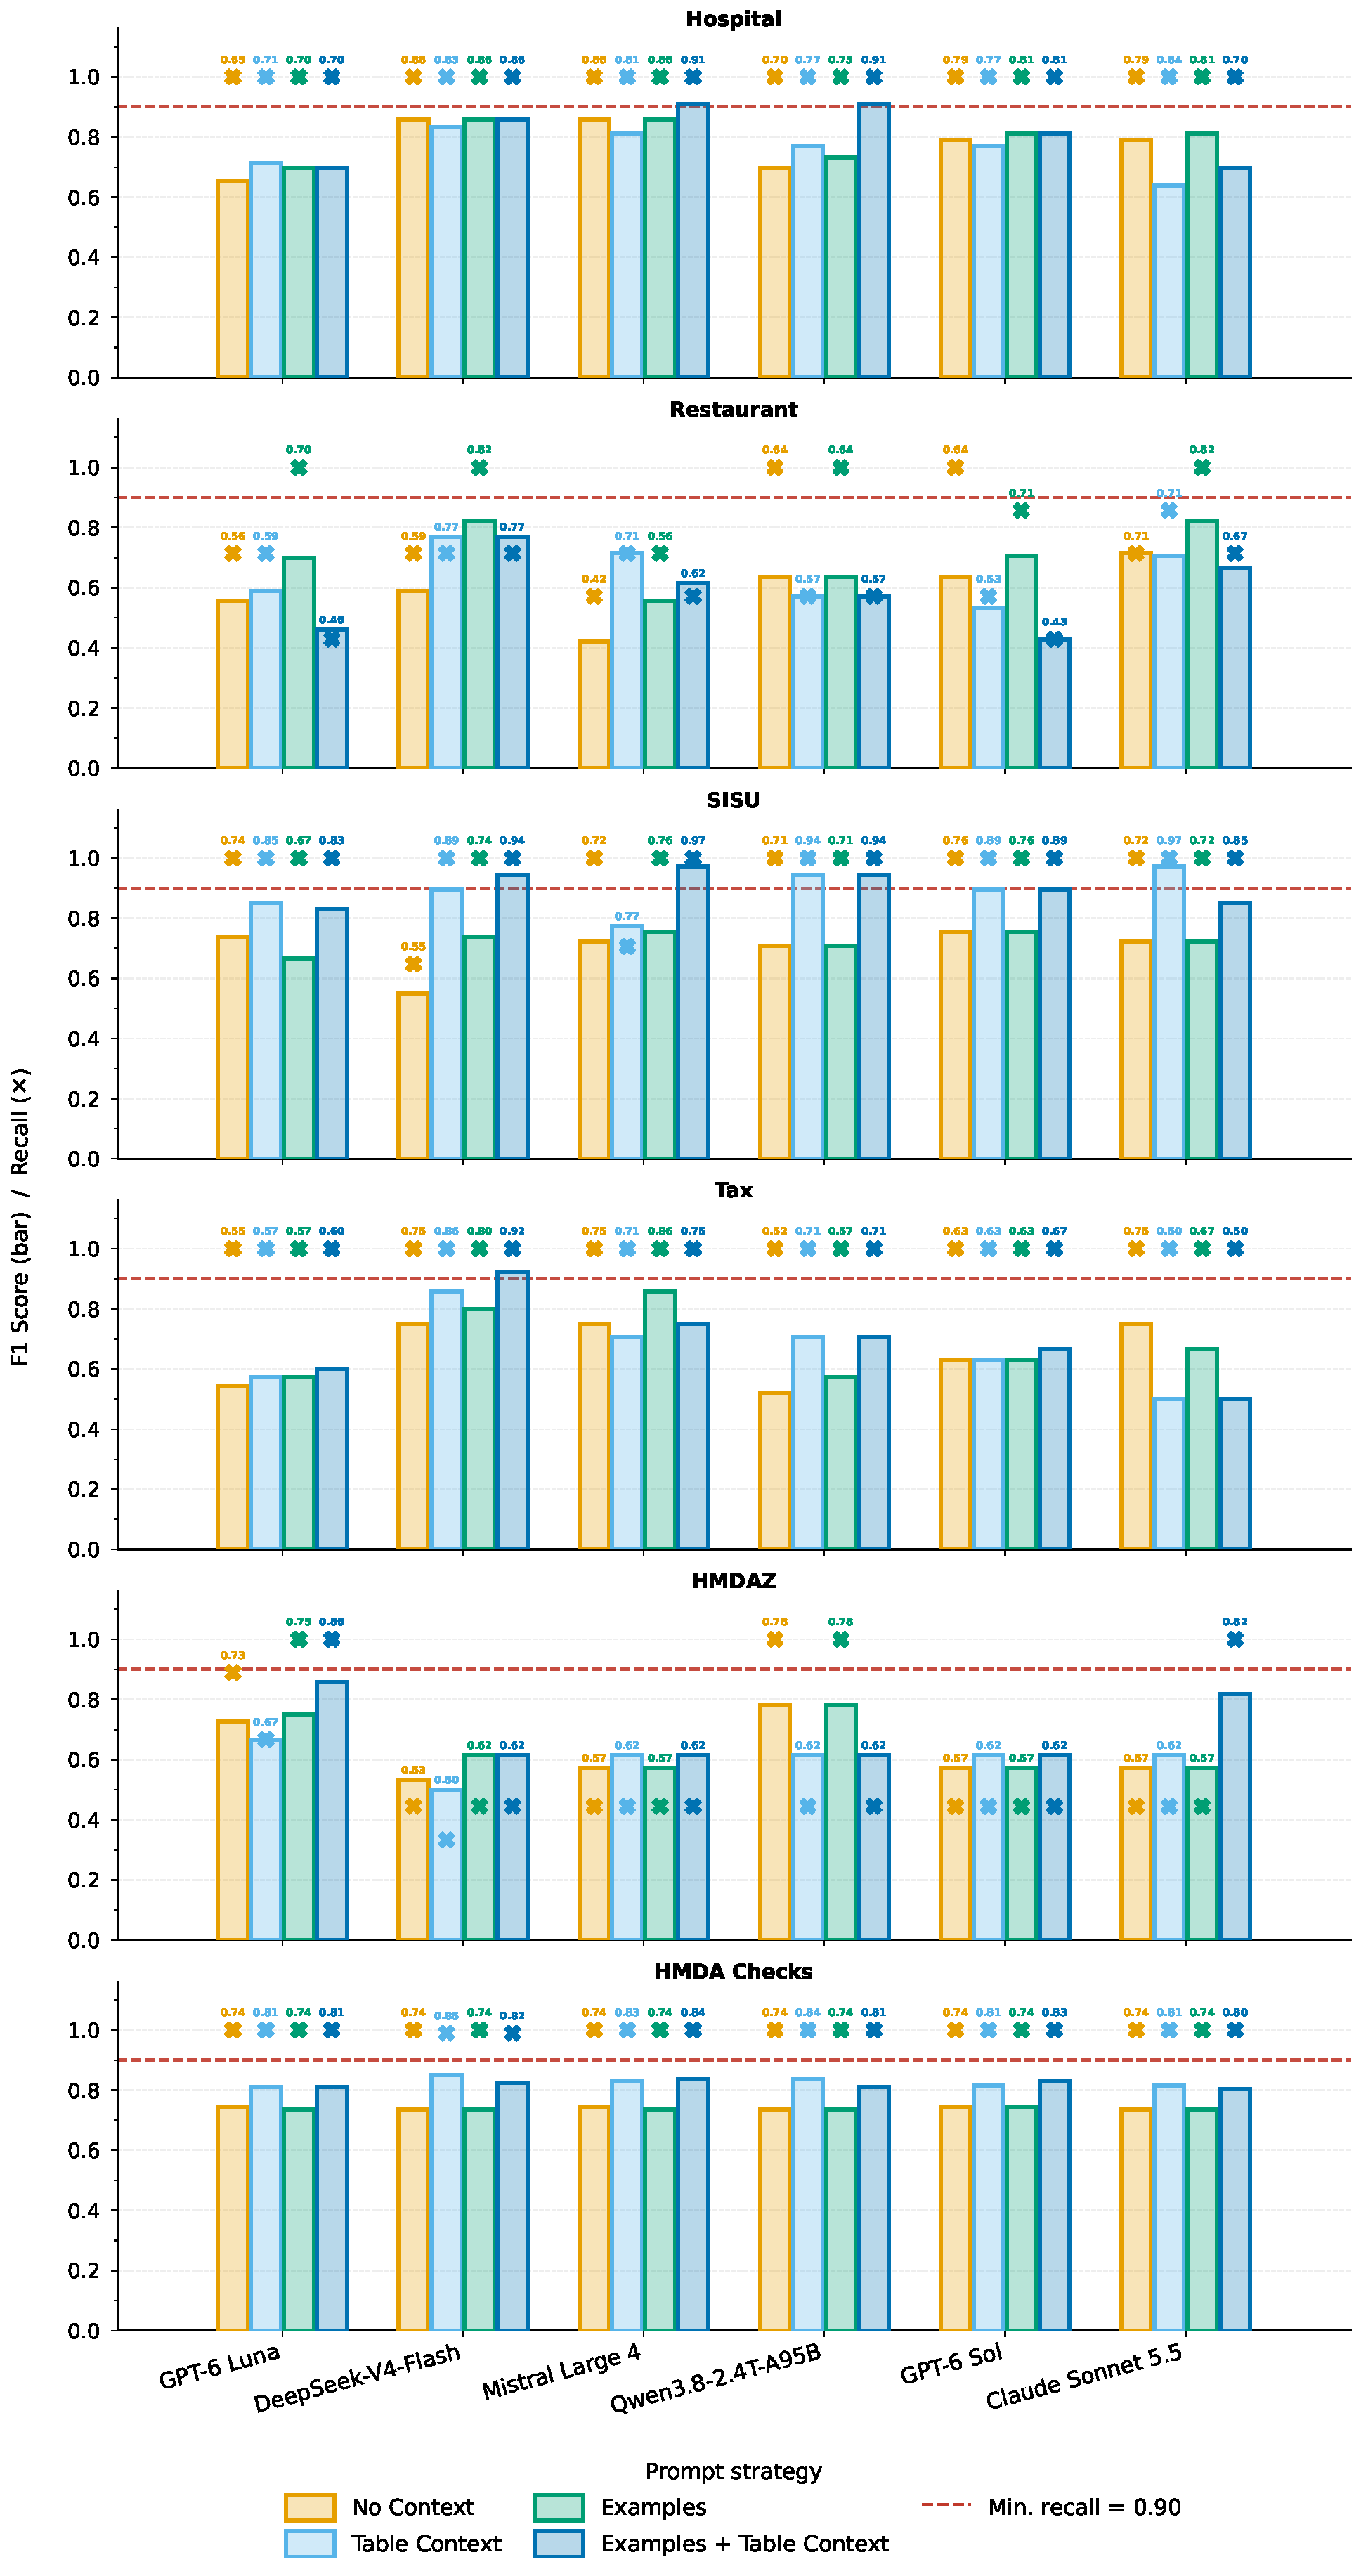
\includegraphics[width=\columnwidth]{figures/results/v3_fig6_classifiers.pdf}
\caption{Constraint classification F$_1$ (bars) and recall (\textsf{x}) across models and prompt variants. The dashed line marks the 0.90 recall threshold.}
    \label{fig:classifier-results}
\end{figure}

On Hospital, Tax, SISU, and HMDA Checks, almost every configuration reaches recall
1.00, so the differences lie in precision. HMDAZ and Restaurant behave
differently: there, recall is the bottleneck. On HMDAZ, most configurations
recover only 4 of the 9 constraint sentences (recall 0.44). The missed sentences
are regulatory definitions (e.g., when a mortgage is high-cost) that read as
scope statements, although each implies a checkable condition on the data. Only three configurations satisfy the recall requirement on all six datasets:
\emph{Qwen3.8-2.4T-A95B} with \emph{Examples} (mean F$_1$ 0.69),
\emph{GPT-6 Luna} with \emph{Examples} (0.69), and \emph{Qwen3.8-2.4T-A95B} with
\emph{No Context} (0.68). \subs{As in our previous evaluation, the}{The} qualifying configurations
are dominated by \emph{Examples}, and we select \emph{Qwen3.8-2.4T-A95B} with
\emph{Examples} as the default classifier. Configurations with higher mean F$_1$
exist (e.g., DeepSeek-V4-Flash with \emph{Examples + Table Context}, 0.82), but
they miss more than half of the HMDAZ constraints.

Table context has two opposite effects. It is the only signal that raises
precision on HMDA Checks: without it, the models label (almost) every edit as a
constraint, and F$_1$ equals that of the trivial all-positive classifier (0.74).
The non-constraint edits are phrased like the checkable ones \subs{and differ
only in that they refer to aggregates, the transmittal sheet, or external
reference data; we conjecture that the record layout shown in the table context
is what lets the model tell them apart.}{but refer to aggregates or external data, which the record layout in the table context presumably exposes.} With table context, F$_1$ rises
to 0.80--0.85. On wide schemas, however, the same context does not
help recall: on HMDAZ (135 columns), 9 of the 12 table-context configurations
stay at or below 0.44, and only GPT-6 Luna and Claude Sonnet 5.5 with
\emph{Examples + Table Context} recover all nine constraint sentences. Averaged over all models and datasets, \emph{Examples} gives the best recall (0.93), while the table-context variants give higher precision (0.71 vs.\ 0.58--0.62) at the cost of recall (0.85--0.87).

\subs{Compared with the backbones of our previous evaluation, the current models are, on average, better classifiers on the four original datasets (mean F$_1$ 0.72 vs.\ 0.69 across all configurations), but the best configuration that satisfies the recall constraint is weaker (0.66 on those four datasets vs.\ 0.85 for Qwen3-32B with \emph{Examples}). Newer models tend to accept more sentences as constraints, which keeps recall high but lowers precision, especially on Tax and Restaurant.}{Compared with earlier backbones that we evaluated with the same protocol in a preliminary study (e.g., Qwen3-32B and GPT-5), the current models are better on average on Hospital, Restaurant, SISU, and Tax (mean F$_1$ 0.72 vs.\ 0.69), but they accept more non-constraint sentences, so the best qualifying configuration is weaker (0.66 vs.\ 0.85 for Qwen3-32B with \emph{Examples}).}
\add{Without examples or table context, classification is already strong on the two controlled datasets (recall 1.00 and mean F$_1$ 0.72 on Tax and Hospital), and the best prompt variant adds only 0.04 on average. On SISU, Restaurant, and the two HMDA datasets, the gain is larger (mean F$_1$ from 0.66 to 0.75 with \emph{Examples + Table Context}), mostly through precision; the GPT-6 models gain the least (0.03--0.05). A plausible explanation is that the LLM-written controlled sentences resemble text these models produce or saw in pretraining; we cannot verify such exposure, but the larger gains on real regulatory text suggest that context matters most there.}
 
\subsection{Constraint Mapping Performance}
\label{sec:constraintextraction}

Our second experiment evaluates how model and mapper choices affect mapping
quality. We evaluate mapping quality using \emph{constraint mapping} F$_1$ and \emph{aggregate
violation} F$_1$ as metrics. To isolate mapper quality from
classification errors, both metrics are computed only on the ground-truth
constraint sentences. We compare the \emph{Single-Prompt} and \emph{Multi-Step}
mappers across six LLMs on all six datasets.

\subs{Figure~\mbox{\ref{fig:mapper-results}} summarizes the results. On the four original
datasets, \emph{Multi-Step} again improves both constraint extraction and
aggregate violation recovery over \emph{Single-Prompt} (mean over models:
0.80 vs.\ 0.75 and 0.89 vs.\ 0.55). The largest gains are on Restaurant and
SISU, whose rules combine several conditions or relate two tuples. Hospital and
Tax are easy for most configurations. With the current backbones, the best
Multi-Step configurations exceed the best configuration of the preliminary study (GPT-5, 0.78 extraction and 0.95 violation): Claude Sonnet 5.5 reaches
0.84 and 0.97, and GPT-6 Sol and Mistral Large 4 0.81 and 0.99.}{Figure~\ref{fig:mapper-results} summarizes the results. On Hospital, Restaurant, SISU, and Tax, \emph{Multi-Step} again improves both constraint mapping and aggregate violation recovery over \emph{Single-Prompt} (mean over models: 0.81 vs.\ 0.75 and 0.83 vs.\ 0.55). The largest gains are on Restaurant and SISU, whose rules combine several conditions or relate two tuples. Hospital and Tax are easy for most configurations. With the current backbones, the best Multi-Step configurations exceed the best configuration of the preliminary study (GPT-5, 0.78 mapping and 0.95 violation): Claude Sonnet 5.5 reaches 0.85 and 0.97, GPT-6 Luna 0.82 and 0.98, and Qwen3.8-2.4T-A95B 0.80 and 1.00.} Decomposition also keeps the mapper
usable when a backbone is unstable under the single-prompt formulation: a
backbone we initially included, MiniMax-M3, returned empty outputs for most
Single-Prompt batches (107 of 156 sentences counted as output failures) but
completed the Multi-Step pipeline without failures; we replaced it with Mistral
Large 4, and among the six final backbones only DeepSeek-V4-Flash has output
failures (3 Single-Prompt sentences).

\begin{figure}[!ht]
    \centering
    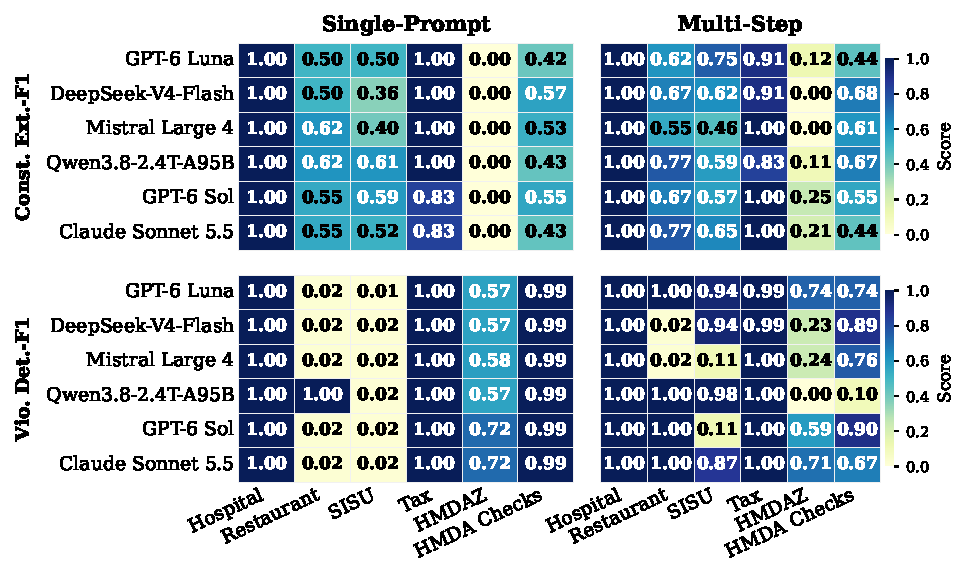
\includegraphics[width=\columnwidth]{figures/results/v3_fig7_mapping.pdf}
    \caption{Sentence-level mapping results across models and mappers, measured by constraint mapping F$_1$ and aggregate violation F$_1$ on ground-truth sentences only.}
    \label{fig:mapper-results}
\end{figure}

\smallskip\noindent\textbf{Where Single-Prompt loses violations.}
The aggregate gap on Restaurant and SISU has two distinct causes. On Restaurant,
one rule (at least one inspection per year) flags 99\% of the gold-violating
tuples. Every Single-Prompt configuration except Qwen3.8-2.4T-A95B returns
\texttt{null} for it, so aggregate recall falls to 0.01. Once this rule is
excluded, all of them reach 1.00. On SISU, the Single-Prompt mapper identifies
the student by the exam registration number instead of the national ID in the
two-tuple rules. The resulting DCs flag about 51k tuples instead of 533
(precision below 0.01)\rem{, although most single-tuple rules are correct}. Multi-Step avoids both errors \add{with most backbones }because it links columns
and selects predicates before writing the DC\add{, but not with all of them: DeepSeek-V4-Flash and Mistral Large 4 also miss the Restaurant rule, and GPT-6 Sol and Mistral Large 4 make the same identification error on SISU in one rule (8.9k tuples; aggregate 0.11)}.

\smallskip\noindent\textbf{HMDA datasets.}
\subs{The two HMDA datasets remain the hardest. Exact extraction stays low (at most
0.24 on HMDAZ and 0.68 on HMDA Checks), mainly for two reasons. Many predicted
DCs are logically equivalent to the gold ones but written differently, e.g.,
\texttt{IN} instead of a disjunction, or a label column instead of its code
column. Others omit the coverage conditions of a trigger. Equivalence-aware
extraction (Table~\mbox{\ref{tab:mapping-metrics}}) recovers a large part of the first
group: on the HMDA datasets it raises the mean extraction F$_1$ from 0.36 to
0.49 for Multi-Step and from 0.24 to 0.51 for Single-Prompt. On the four original
datasets it is almost identical to exact extraction. The aggregate violation
ranking is also reversed on HMDA Checks: Single-Prompt reaches 0.99, while
Multi-Step stays at 0.10--0.16. This reversal says little about mapping quality.
Two date-range edits (S270 and Q022) flag 99\% of the gold-violating tuples, which
cover 98.6\% of the rows, so a DC that flags \emph{every} tuple already scores 0.99.
These are the only gold DCs that need arithmetic over dates encoded as integers.
Multi-Step returns \texttt{null} for both with every backbone, consistent with its
precision bias. Single-Prompt writes DCs for them, but most of these DCs flag all
rows (e.g., \texttt{t1.action\_taken\_date / 10000 != t1.activity\_year}, which
never holds as an equality under real division); only GPT-6 Luna, GPT-6 Sol, and
Qwen3.8-2.4T-A95B produce an execution-equivalent DC for one of the two. Without these
two edits, the ranking flips back: Multi-Step reaches 1.00 with Claude Sonnet 5.5,
GPT-6 Luna, and GPT-6 Sol and 0.77 with the other three backbones (mean 0.89),
whereas Single-Prompt ranges from 0.18 to 1.00 (mean 0.65). Per-rule metrics,
which weigh every rule equally, are far less sensitive to these two edits: on
HMDA Checks, the mean per-rule violation F$_1$ is 0.80 for Multi-Step and 0.86 for
Single-Prompt with all edits, and 0.87 and 0.85 without the date edits. On the
remaining rules, the two mappers are therefore close, and the aggregate
reversal does not reflect the overall quality of the rules.}{The two HMDA datasets remain the hardest. Exact mapping stays low (at most 0.25 on HMDAZ and 0.68 on HMDA Checks), mainly for two reasons. Many predicted DCs are logically equivalent to the gold ones but written differently, e.g., \texttt{IN} instead of a disjunction, or a label column instead of its code column. Others omit the coverage conditions of a trigger. Equivalence-aware mapping (Table~\ref{tab:mapping-metrics}) recovers a large part of the first group: on the HMDA datasets it raises the mean mapping F$_1$ from 0.34 to 0.46 for Multi-Step and from 0.24 to 0.51 for Single-Prompt, whereas on the other datasets it is almost identical to exact mapping. On HMDA Checks, aggregate violation is not informative. Two date-range edits flag 99\% of the gold-violating tuples, which cover 98.6\% of the rows, so a DC that flags every tuple already scores 0.99. Single-Prompt reaches 0.99 with every backbone, mostly through such DCs. Multi-Step scores 0.67--0.90 with five backbones, but only GPT-6 Sol maps one of the date edits correctly; the others write incorrect DCs for other edits that flag 480k--550k rows and pass the 90\% violation-share check. Without the two date edits, these broad DCs are exposed: the Multi-Step aggregate falls to 0.12--0.19 for those four backbones and stays at 0.98--1.00 for GPT-6 Sol and Qwen3.8-2.4T-A95B, while Single-Prompt ranges from 0.18 to 1.00. Per-rule metrics, which weigh every rule equally, are far less sensitive: the mean per-rule violation F$_1$ is 0.78 for Multi-Step and 0.86 for Single-Prompt with all edits, and 0.84 and 0.85 without the date edits.}

\begin{table}[!ht]
  \centering
  \small
  \setlength{\tabcolsep}{3.5pt}
  \resizebox{\columnwidth}{!}{\begin{tabular}{llrrrrrr}
\toprule
\textbf{Mapper} & \textbf{Model} & CM & CM$_{\equiv}$ & AV & Rule-F$_1$ & Exec. & Fail. \\
\midrule
\multirow{6}{*}{Single-Prompt} & GPT-6 Luna & 0.57 & 0.69 & 0.60 & 0.78 & 0.75 & 0 \\
 & DeepSeek-V4-Flash & 0.57 & 0.66 & 0.60 & 0.74 & 0.70 & 3 \\
 & Mistral Large 4 & 0.59 & 0.66 & 0.60 & 0.73 & 0.71 & 0 \\
 & Qwen3.8-2.4T-A95B & 0.61 & 0.70 & 0.76 & \textbf{0.86} & \textbf{0.83} & 0 \\
 & GPT-6 Sol & 0.59 & 0.67 & 0.62 & 0.76 & 0.72 & 0 \\
 & Claude Sonnet 5.5 & 0.55 & 0.64 & 0.62 & 0.76 & 0.70 & 0 \\
\midrule
\multirow{6}{*}{Multi-Step} & GPT-6 Luna & 0.64 & 0.69 & \textbf{0.90} & 0.77 & 0.76 & 0 \\
 & DeepSeek-V4-Flash & 0.65 & 0.69 & 0.68 & 0.68 & 0.69 & 0 \\
 & Mistral Large 4 & 0.60 & 0.64 & 0.52 & 0.74 & 0.73 & 0 \\
 & Qwen3.8-2.4T-A95B & 0.66 & 0.68 & 0.68 & 0.81 & 0.77 & 0 \\
 & GPT-6 Sol & 0.67 & 0.71 & 0.77 & 0.79 & 0.77 & 0 \\
 & Claude Sonnet 5.5 & \textbf{0.68} & \textbf{0.74} & 0.88 & 0.84 & 0.82 & 0 \\
\bottomrule
\end{tabular}
}
  \caption{Mean mapping quality over the six datasets (ground-truth sentences
  only). CM: exact mapping F$_1$; CM$_{\equiv}$: equivalence-aware mapping
  F$_1$; AV: aggregate violation F$_1$; Rule-F$_1$: mean per-rule violation F$_1$;
  Exec.: execution equivalence; Fail.: sentences with no valid model output.}
  \label{tab:mapping-metrics}
\end{table}

\subs{\smallskip\noindent\textbf{Default mapper.}
No single model leads on both metrics of the paper protocol: across the six
datasets, Qwen3.8-2.4T-A95B has the best mean extraction (0.68) and Mistral
Large 4 the best mean aggregate violation (0.80) with Multi-Step. We therefore use the mean of the two to break the tie and select
\emph{GPT-6 Sol} with \emph{Multi-Step} (0.67 and 0.78; mean 0.727, against 0.722 for
Mistral Large 4, 0.718 for Claude Sonnet 5.5, and 0.707 for Qwen3.8-2.4T-A95B) as the default
sentence-level configuration. Differences among these four are within the variation that a single
run per configuration can show, so the choice should be read as a tie among
them rather than a clear winner.}{\smallskip\noindent\textbf{Default mapper.}
No single model leads on both metrics of the paper protocol: across the six datasets, Claude Sonnet 5.5 has the best mean mapping (0.68) and GPT-6 Luna the best mean aggregate violation (0.90) with Multi-Step. We use the mean of the two to break the tie and select \emph{Claude Sonnet 5.5} with \emph{Multi-Step} (mean 0.776, against 0.771 for GPT-6 Luna and 0.720 for GPT-6 Sol) as the default sentence-level configuration. With a single run per configuration, this is a tie with GPT-6 Luna.}

\add{\smallskip\noindent\textbf{Sensitivity to the backbone.}
Backbones differ more in violation detection than in mapping. With Multi-Step, mean exact mapping ranges only from 0.60 (Mistral Large 4) to 0.68 (Claude Sonnet 5.5), whereas aggregate violation ranges from 0.52 to 0.90; per-rule metrics lie in between (0.68--0.84) and rank Claude Sonnet 5.5, Qwen3.8-2.4T-A95B, and GPT-6 Sol highest. The divergences concentrate on implicit decisions rather than on syntax: which attribute identifies an entity (SISU), whether a definition implies a checkable trigger (HMDAZ), and how integer-encoded dates are compared (HMDA Checks). Finally, single runs vary: in two runs of Mistral Large 4 on Restaurant that differ only in a check that does not affect the dominant rule, the aggregate went from 1.00 to 0.02, because that rule was mapped in one run and not in the other. We cannot relate these differences to model size or training data, which are not disclosed for most backbones.}

 
\subsection{End-to-End Evaluation and Comparison}
\label{sec:endtoend}

We now evaluate the full Text-to-Constraints pipeline end-to-end and compare \system\ against the baselines from Section~\ref{sec:baselines}. For \system, we use the default components selected in the previous experiments: \emph{Qwen3.8-2.4T-A95B} with \emph{Examples} for constraint classification and \subs{\emph{GPT-6 Sol}}{\emph{Claude Sonnet 5.5}} with \emph{Multi-Step} for mapping.
We report two variants of \system: \subs{(1) the full pipeline, which combines the first-stage constraint classifier with the Multi-Step mapper (C+MS), and (2) the Multi-Step mapper alone, which skips the initial classification stage and relies on its own rule filter (Multi-Step).}{the full pipeline with the classifier and the Multi-Step mapper (C+MS), and the Multi-Step mapper alone, which relies on its own rule filter (Multi-Step).}
As baselines, we include (i) the best result from DC discovery, following the procedure previously described, and (ii) an adaptation of the Text-to-SQL tool XiYan-SQL, as described before. Baseline results on \subs{the four original datasets are those of our previous evaluation}{Hospital, Restaurant, SISU, and Tax come from the preliminary study (Section~\ref{sec:constraintdetection})}, which used the same data and gold constraints\add{ (their SISU violation scores predate the pair semantics of Section~\ref{sec:mapper:sql})}; the baselines were not run on the HMDA datasets.
\add{Each end-to-end configuration is executed three times, and Table~\ref{tab:main_results} reports the mean for \system. }Table~\ref{tab:main_results} shows the results on all six datasets using the three metrics introduced in Section~\ref{sec:metrics}: constraint classification, constraint extraction, and violation detection.

\begin{table}[!ht]
  \centering
  \small
  \setlength{\tabcolsep}{4pt}
  \resizebox{\columnwidth}{!}{%
  \begin{tabular}{llccccccccc}
\toprule
\textbf{Family} & \textbf{Method} & \multicolumn{3}{c}{Constr. Classification} & \multicolumn{3}{c}{Constr. Extraction} & \multicolumn{3}{c}{Viol. Detection} \\
\cmidrule(lr){3-5}  \cmidrule(lr){6-8}  \cmidrule(lr){9-11}
 &  & P & R & F$_1$ & P & R & F$_1$ & P & R & F$_1$ \\
\midrule
\addlinespace[2pt]
\multicolumn{11}{c}{\textbf{Hospital}} \\
\addlinespace[1pt]
\multirow{2}{*}{\system} & ~~C+MS & 0.81 & 1.00 & \textbf{0.89} & 1.00 & 1.00 & \textbf{1.00} & 1.00 & 1.00 & \textbf{1.00} \\
 & ~~Multi-Step & 0.48 & 1.00 & 0.65 & 1.00 & 1.00 & \textbf{1.00} & 1.00 & 1.00 & \textbf{1.00} \\
\cmidrule(l){2-11}
\multirow{1}{*}{Profiling} & ~~DC Discovery & n/a & n/a & n/a & 0.00 & 0.00 & 0.00 & 0.83 & 1.00 & 0.91 \\
\cmidrule(l){2-11}
\multirow{1}{*}{Text2SQL} & ~~XiYan-SQL & 0.50 & 1.00 & 0.67 & 0.60 & 1.00 & 0.75 & 0.83 & 1.00 & 0.91 \\
\midrule
\addlinespace[2pt]
\multicolumn{11}{c}{\textbf{Restaurant}} \\
\addlinespace[1pt]
\multirow{2}{*}{\system} & ~~C+MS & 0.89 & 0.71 & 0.79 & 0.80 & 0.57 & \textbf{0.67} & 1.00 & 0.34 & 0.35 \\
 & ~~Multi-Step & 0.65 & 0.71 & 0.68 & 0.80 & 0.57 & \textbf{0.67} & 0.87 & 0.01 & 0.02 \\
\cmidrule(l){2-11}
\multirow{1}{*}{Profiling} & ~~DC Discovery & n/a & n/a & n/a & 0.00 & 0.00 & 0.00 & 0.77 & 0.87 & \textbf{0.82} \\
\cmidrule(l){2-11}
\multirow{1}{*}{Text2SQL} & ~~XiYan-SQL & 0.86 & 0.75 & \textbf{0.80} & 0.17 & 0.12 & 0.14 & 0.45 & 0.64 & 0.52 \\
\midrule
\addlinespace[2pt]
\multicolumn{11}{c}{\textbf{SISU}} \\
\addlinespace[1pt]
\multirow{2}{*}{\system} & ~~C+MS & 0.67 & 1.00 & \textbf{0.80} & 0.65 & 0.65 & \textbf{0.65} & 0.03 & 0.98 & \textbf{0.06} \\
 & ~~Multi-Step & 0.65 & 1.00 & 0.79 & 0.65 & 0.65 & \textbf{0.65} & 0.03 & 0.97 & 0.05 \\
\cmidrule(l){2-11}
\multirow{1}{*}{Profiling} & ~~DC Discovery & n/a & n/a & n/a & 0.00 & 0.00 & 0.00 & 0.00 & 0.99 & 0.01 \\
\cmidrule(l){2-11}
\multirow{1}{*}{Text2SQL} & ~~XiYan-SQL & 1.00 & 0.65 & 0.79 & 0.45 & 0.29 & 0.36 & 0.00 & 1.00 & 0.01 \\
\midrule
\addlinespace[2pt]
\multicolumn{11}{c}{\textbf{Tax}} \\
\addlinespace[1pt]
\multirow{2}{*}{\system} & ~~C+MS & 0.71 & 1.00 & \textbf{0.82} & 1.00 & 1.00 & \textbf{1.00} & 0.59 & 1.00 & \textbf{0.70} \\
 & ~~Multi-Step & 0.33 & 1.00 & 0.50 & 1.00 & 1.00 & \textbf{1.00} & 0.01 & 1.00 & 0.02 \\
\cmidrule(l){2-11}
\multirow{1}{*}{Profiling} & ~~DC Discovery & n/a & n/a & n/a & 0.00 & 0.00 & 0.00 & 0.00 & 0.94 & 0.01 \\
\cmidrule(l){2-11}
\multirow{1}{*}{Text2SQL} & ~~XiYan-SQL & 0.40 & 1.00 & 0.57 & 0.29 & 0.67 & 0.40 & 0.01 & 1.00 & 0.02 \\
\midrule
\addlinespace[2pt]
\multicolumn{11}{c}{\textbf{HMDAZ}} \\
\addlinespace[1pt]
\multirow{2}{*}{\system} & ~~C+MS & 0.86 & 0.89 & 0.87 & 0.13 & 0.15 & 0.14 & 0.26 & 1.00 & 0.38 \\
 & ~~Multi-Step & 0.96 & 0.89 & \textbf{0.92} & 0.25 & 0.26 & \textbf{0.25} & 0.48 & 1.00 & \textbf{0.64} \\
\cmidrule(l){2-11}
\multirow{1}{*}{Profiling} & ~~DC Discovery & -- & -- & -- & -- & -- & -- & -- & -- & -- \\
\cmidrule(l){2-11}
\multirow{1}{*}{Text2SQL} & ~~XiYan-SQL & -- & -- & -- & -- & -- & -- & -- & -- & -- \\
\midrule
\addlinespace[2pt]
\multicolumn{11}{c}{\textbf{HMDA Checks}} \\
\addlinespace[1pt]
\multirow{2}{*}{\system} & ~~C+MS & 0.90 & 0.93 & 0.91 & 0.45 & 0.43 & 0.44 & 0.99 & 0.56 & \textbf{0.71} \\
 & ~~Multi-Step & 0.90 & 0.93 & \textbf{0.92} & 0.45 & 0.44 & \textbf{0.45} & 0.99 & 0.56 & \textbf{0.71} \\
\cmidrule(l){2-11}
\multirow{1}{*}{Profiling} & ~~DC Discovery & -- & -- & -- & -- & -- & -- & -- & -- & -- \\
\cmidrule(l){2-11}
\multirow{1}{*}{Text2SQL} & ~~XiYan-SQL & -- & -- & -- & -- & -- & -- & -- & -- & -- \\
\bottomrule
\end{tabular}

  }%
\caption{End-to-end comparison of \system\ modes, Classifier+Multi-Step (C+MS) and Multi-Step, and the baselines across six
datasets\add{ (\system: mean of three runs)}. \textbf{Profiling} denotes DC discovery from data alone, and
\textbf{Text2SQL} denotes XiYan-SQL adapted to generate violation queries from
regulatory sentences; their results on \subs{the four original datasets come from our
previous evaluation}{Hospital, Restaurant, SISU, and Tax come from the preliminary study}, and -- marks configurations not run. n/a indicates that the metric is not applicable; bold
marks the best F$_1$ for each metric and dataset.}
  \label{tab:main_results}
\end{table}

\subs{\system\ is the only approach that produces gold constraints on every dataset.
Constraint extraction F$_1$ is 1.00 on Hospital and Tax, 0.67 on Restaurant,
0.53--0.59 on SISU, 0.58--0.59 on HMDA Checks, and 0.24--0.40 on HMDAZ, against
at most 0.75 for XiYan-SQL and zero for DC discovery on the original datasets.
Classification is also strong, with F$_1$ between 0.75 and 0.92 for C+MS. The
pipeline therefore extends to the two HMDA datasets, with up to 135 columns and
1M rows, against at most 56 columns and 128k rows in the original ones. On
HMDA Checks, the 92 constraint edits are classified with F$_1$ 0.92 and more than
half of them are extracted exactly.}{\system\ is the only approach that produces gold constraints on every dataset.
Constraint extraction F$_1$ is 1.00 on Hospital and Tax, 0.67 on Restaurant, 0.65 on SISU, 0.44--0.45 on HMDA Checks, and 0.14--0.25 on HMDAZ (0.35 with equivalence-aware matching), against at most 0.75 for XiYan-SQL and zero for DC discovery. Classification is also strong, with F$_1$ between 0.79 and 0.91 for C+MS. The pipeline therefore extends to the two HMDA datasets, with up to 135 columns and 1M rows, against at most 56 columns and 128k rows in the other datasets.}

\subs{The classifier mainly improves precision. Compared with \emph{Multi-Step} alone,
\emph{C+MS} raises classification precision on Hospital (0.83 vs.\ 0.71), SISU
(0.84 vs.\ 0.75), and HMDA Checks (0.94 vs.\ 0.92), and it reduces the
non-constraint sentences that reach a DC (3 vs.\ 6 on Hospital, 3 vs.\ 5 on SISU,
5 vs.\ 7 on HMDA Checks). With the current backbones, however, the gain is
smaller than with the earlier backbones. The Multi-Step rule filter already
rejects most non-constraint sentences, and on Restaurant, Tax, and HMDAZ both
variants make the same classification decisions. On HMDAZ, C+MS is worse on
extraction and violations (0.24 vs.\ 0.40 and 0.56 vs.\ 0.72). The two variants
map five common sentences and differ on one each: the classifier drops the
balloon-payment limitation, which Multi-Step maps exactly, and keeps the
points-and-fees trigger, which the Multi-Step filter rejects. The two runs also
write different DCs for the APR trigger (per-rule violation F$_1$ 0.17 vs.\
0.35). Part of the gap is therefore run-to-run variation of a single execution.}{The classifier mainly improves precision. Compared with \emph{Multi-Step} alone, \emph{C+MS} raises classification precision on Hospital (0.81 vs.\ 0.48), Restaurant (0.89 vs.\ 0.65), and Tax (0.71 vs.\ 0.33). On Tax, this decides the aggregate violation score. Multi-Step alone maps about 12 non-constraint sentences per run, which were written to resemble constraints, to DCs; one of them turns ``major cities exist within fixed states'' into \texttt{t1.city = t2.city AND t1.state != t2.state}, which flags 52k tuples, so the aggregate falls to 0.02. C+MS filters most of them and reaches 0.70 on average (0.55--1.00). On the two HMDA datasets, both variants make almost the same decisions; on HMDAZ, they nevertheless write different DCs for the same triggers (mean exact extraction 0.14 vs.\ 0.25, equivalence-aware 0.35 for both), and the aggregate varies from 0.02 to 0.75 across runs.}

\subs{The violation results expose two failure modes that are specific to the
end-to-end setting, where non-constraint sentences can also reach the mapper.
On Tax, every gold constraint is extracted exactly (F$_1$ 1.00), yet aggregate
violation F$_1$ falls to 0.15. Four of the 120 non-constraint sentences are
accepted by the classifier and the rule filter and mapped to DCs. These
sentences were written to resemble constraints (e.g., ``The sample data shows
exemption values ranging from \$0 to \$6,600, all falling well within respective
salary figures''), and the resulting DCs flag 5.6k tuples against 468 gold
violations. On SISU, the C+MS run maps one gold sentence with an additional
two-tuple rule that identifies students by exam registration instead of national
ID, so that the run flags 9.2k tuples against 533 gold violations (aggregate F$_1$ 0.11 vs.\ 0.87 for Multi-Step, whose
DC for the same sentence uses the national ID). Both cases show that a single broad DC dominates the tuple-level
aggregate. On HMDA Checks, the aggregate (0.10) again reflects the two date-range
edits discussed in Section~\mbox{\ref{sec:constraintextraction}}. The per-rule view is
more informative there: 83\% of the gold rules with violations are reproduced
exactly (execution equivalence 0.83 for both variants), and the mean per-rule
violation F$_1$ is 0.80--0.83.}{The violation results expose two further failure modes. First, a broad DC on a non-constraint sentence can dominate the aggregate. On SISU, both variants map sentences that define quota categories, which our ground truth labels as non-constraints, to checks between two quota attributes that flag up to 12k tuples; the aggregate stays at 0.05--0.06, although the gold rules are recovered well (per-rule violation F$_1$ 0.91--0.95, execution equivalence 0.86--0.90). Second, missing a dominant rule: on Restaurant, the yearly-inspection rule flags 99\% of the gold violations, and Multi-Step alone returns no DC for it in all three runs, C+MS in two of them. The rule filter judges this requirement, which concerns inspections across years, as not expressible, although the derived attribute encodes it. The aggregate is therefore 0.02 for Multi-Step and 0.35 on average for C+MS, below DC discovery (0.82), while extraction reaches 0.67. Both failures depend on the backbone and the run: with GPT-6 Sol as the mapper, the pipeline reached 1.00 on Restaurant and up to 0.98 on SISU but 0.15 on Tax. On HMDA Checks, the aggregate of 0.71 is not evidence of quality: no date-range edit is mapped, and the score comes from an incorrect DC that flags 481k tuples, most of which violate some gold rule. The per-rule view is more informative there: 83\% of the gold rules with violations are reproduced exactly, and the mean per-rule violation F$_1$ is 0.77--0.78.}

The baselines are competitive only on narrower parts of the experiments\rem{, that is, on specific aspects of the evaluation}. The profiling baseline can recover meaningful violation signals when the data distribution strongly reflects the target rules, but it does not recover the gold
constraint set itself, with constraint-extraction F$_1$ equal to zero on all datasets. XiYan-SQL is competitive on Hospital, but its behavior is much less reliable on the remaining datasets. On SISU and Tax in particular, it achieves very high recall for violations but near-zero precision, indicating that it returns queries pointing to overly broad violation sets.

Finally, the dataset characteristics matter when interpreting the aggregate
violation results. In four of the six datasets, a single gold rule flags most of
the gold-violating tuples\rem{ (96\% on Hospital, 99\% on Restaurant, 78\% on Tax, and
99\% on HMDA Checks)}\add{ (Section~\ref{sec:constraintextraction})}. \rem{The aggregate then mostly measures whether that rule is
recovered. }Methods that return broad violation sets can still overlap strongly
with the gold violations, as with the profiling baseline on Hospital and
Restaurant. Conversely, a correct pipeline can be penalized by one broad false
positive, as on Tax\add{ and SISU}. We therefore recommend reading the aggregate together with
the per-rule metrics of Section~\ref{sec:metrics}.
Overall, \system\ is the only approach that remains strong on classification and extraction across all six datasets\add{; it is behind the baselines only on Restaurant, in violation detection and, by 0.01, in classification}. The violation metric remains sensitive to individual broad DCs.

\add{\smallskip\noindent\textbf{Usability of the output.} The returned set stays small and reviewable: C+MS returns 6--25 DCs per run on Hospital, Restaurant, SISU, and Tax, 9 on HMDAZ, and 95 on HMDA Checks, close to the number of gold constraints (6--92). Users can rank the DCs by the number of tuples they flag, read the source sentence of each one, and use the optional review step of the pipeline (Section~\ref{sec:overview}); the broad DCs discussed above stand out precisely by their violation counts.}


\smallskip\noindent\textbf{Costs.}
\subs{The full sentence-level \system\ pipeline is the most expensive variant because it requires multiple model calls per sentence. In this evaluation, all experiments together cost US\$83 through OpenRouter (E1 US\$5.8, E2 US\$52.7, end-to-end US\$24.5). With GPT-6 Sol, an end-to-end run costs between US\$0.3 and US\$2.3 on the original datasets and between US\$3.4 (C+MS) and US\$9.9 (Multi-Step) on HMDA Checks (158 sentences, 1M rows). The classifier makes the pipeline 1.6 to 5 times cheaper, because rejected sentences never reach the Multi-Step mapper. Low-cost backbones such as GPT-6 Luna and DeepSeek-V4-Flash cost a few cents per dataset. Cost scales linearly with the number of sentences, making the approach tractable in practice. By contrast, data profiling baselines face combinatorial search over the schema, and for some datasets we had to restrict the columns considered.}{The full sentence-level \system\ pipeline is the most expensive variant because it requires multiple model calls per sentence. All reported experiments together cost US\$166 through OpenRouter (E1 US\$5.7, E2 US\$52.9, three end-to-end runs US\$107.2). With Claude Sonnet 5.5, an end-to-end run costs between US\$0.4 and US\$2.9 on Hospital, Restaurant, SISU, and Tax and about US\$9.7 on HMDA Checks (158 sentences, 1M rows). The classifier makes the pipeline up to six times cheaper (Tax), because rejected sentences never reach the Multi-Step mapper; on HMDA Checks, where most sentences are constraints, both variants cost the same. Low-cost backbones such as GPT-6 Luna and DeepSeek-V4-Flash cost a few cents per dataset. By contrast, data profiling baselines face combinatorial search over the schema, and for some datasets we had to restrict the columns considered.}
 









%\subsection{Ablations} 

 \section{Related Work}
\label{sec:related}

\noindent\textbf{Data Profiling.}
The closest line of work to \system\ is \emph{data profiling}, which aims to discover constraints directly from data instances~\cite{profSurveyFelix2015,Huhtala1998TANE,Fan2009DiscoverCFD,Papenbrock2016HyFD,Bleifuss2017Hydra,chu2013discovering,Pena2022FastDC,icdePena2024}. This includes formalisms such as functional dependencies, conditional dependencies, and denial constraints (DCs). DCs are particularly relevant in our setting because they subsume keys, FDs, and ordering constraints~\cite{chu2013discovering}, making them expressive enough to capture many cross-tuple rules in regulatory text. Approximate discovery tolerates violations in dirty data~\cite{Pena2019DiscoveryDC,martin2026lima}, user-specific criteria help experts rank discovered rules~\cite{fan2023topk}, and LLMs now propose candidate rules from schemas and samples~\cite{biester2024llmclean,glock2026ledqer,li2026lcats}. Still, all these methods are driven by the observed data. They reveal what the data seems to satisfy, but not whether that pattern is required by policy or regulation. As a result, profiling cannot recover constraints that are already violated in the released data, and discovered DCs often include many spurious constraints~\cite{martin2025false}. Our goal is to recover constraints from normative text and then use them to validate the data.


\smallskip
\noindent\textbf{Data Cleaning.}
Data cleaning systems use constraints, statistical signals, or both to detect and repair errors~\cite{dataerrorsZiawash,chu2013holistic,holoclean,raha2019,peng2022garf,cleaningDeploy2024}, including rules with ML predicates (REEs)~\cite{bao2024rock} and LLM-based detectors~\cite{ni2025zeroed,zhang2024cleaning}. These systems complement our setting. Constraint-based methods are interpretable and auditable, but they assume that the relevant rules are already available. Data-driven methods reduce the need for manual rule specification, but without an external source of truth, they can struggle to distinguish rare valid values from genuine errors~\cite{cleaningDeploy2024}. Our work addresses this missing step of obtaining such rules from regulatory documents. We use DCs over a controlled, schema-derived predicate space as the output formalism, so every constraint is executable and auditable, and, as prior work has shown, DCs can be checked efficiently at scale~\cite{facet2021,liu2024rapidash,youri2024}.

\smallskip
\noindent\textbf{Regulatory NLP.}
A separate line of work uses NLP to analyze regulations and compliance-related documents, for example, by extracting rights and obligations or by checking whether requirement statements comply with legal or policy text~\cite{breaux2006regulatory,kiyavitskaya2008automating,amaral2023nlp,hassani2024rethinking,compliance2025ACMTSEM,masoudifard2024graphrag}. LLMs now extract structured rules from regulations~\cite{guliani2026dejure,hettiarachchi-etal-2025-code,kabzhan2025semantic} and translate financial regulations into compliance code~\cite{li2025compliance2code}, although they still struggle to apply long sets of interdependent rules~\cite{yu2026ruleworld,soni2026tam}. These approaches remain text-centered or target a fixed application model. Our problem starts from similar documents, but we need to connect regulatory statements to a relational schema and translate them into constraints whose violations can be checked in the data.

\smallskip
\noindent\textbf{Text-to-SQL.}
Text-to-SQL is also related, since it maps natural-language input to a SQL query over a database schema~\cite{yu2018spider,picard2021,resdsql2023,pourreza2023din,dail2025,llmTEXT2SQLSurvey2025,redsql2025,XiYanSQL,alrashed2026verification,rabonato2026portuguese}. The difference lies in how the generated logic is used, as Text-to-SQL produces a query that answers a user question on the current database instance, whereas \system\ aims at declarative invariants that should hold for all valid instances of the data. In addition to mapping text to schema elements, as in Text-to-SQL, it must also identify scope conditions and define violation semantics. Closer in output, LLMs generate OCL constraints from specifications of UML models~\cite{abukhalaf2023ocl,attarwala2026ocl}, and Doc2DB systems verify extracted relations against integrity constraints~\cite{zhang2026doc2db}; in both cases, the target schema is designed together with the constraints, whereas \system\ grounds regulatory text in an independently published dataset.
 


 \section{Conclusion}
\label{sec:conclusion}

A constraint inferred from data describes what the data happens to satisfy, whereas a constraint contained in governing text describes what the data is required to satisfy. This distinction \subs{ }{}has received limited attention in database research, even though many published datasets are accompanied by documents that define data quality criteria at some level. 

In this paper, we show that the gap between data and normative text can be addressed automatically. Our results indicate that lightweight classification is sufficient to detect \subs{ }{}most checkable requirements, and that a structured multi-step pipeline grounded in both text and schema can translate them into executable constraints while avoiding hallucinated predicates and literals. 

This enables a new form of validation: \system\ can reveal compliance failures even when they do not manifest as discoverable \subs{pattern}{patterns} in the data. In such settings, the normative document becomes \subs{ }{}part of the data specification, and keeping that specification aligned with evolving text emerges \add{as} a concrete challenge for data management. \add{Because each constraint comes from the text, it remains valid while the regulation is unchanged and can be re-executed, also incrementally~\cite{youri2024}, as the data evolves; only a change in the text requires a new mapping. Our datasets have at most 158 sentences, whereas legal documents often have hundreds, with nested clauses that must first be segmented and resolved; since cost grows linearly with the number of sentences, we expect the pipeline to scale to them, but this remains to be shown.}


 


% next sections


\bibliographystyle{ACM-Reference-Format}
\bibliography{refs}


%\input{text_full/appendix}

\end{document}
